\documentclass[11pt,a4paper]{article}

\usepackage[spanish,es-noshorthands,es-tabla]{babel}
\usepackage{lmodern}
\usepackage[margin=2.4cm]{geometry}
\usepackage{graphicx}
\usepackage{booktabs}
\usepackage{tabularx}
\usepackage{array}
\usepackage{amsmath}
\usepackage{amssymb}
\usepackage{xcolor}
\usepackage{enumitem}
\usepackage{caption}
\usepackage{float}
\usepackage{tikz}
\usetikzlibrary{positioning,arrows.meta}
\usepackage{xurl}
\usepackage[hidelinks]{hyperref}

\definecolor{azul}{HTML}{2A78D6}
\definecolor{tinta}{HTML}{52514E}
\definecolor{fondo}{HTML}{F3F2EF}

\setlist{itemsep=2pt,topsep=4pt}
% Pie de figura en \small (10 pt); el texto dentro de las figuras se dibuja a 7,5--8,5 pt.
\captionsetup{font=small,labelfont=bf}
\newcolumntype{L}{>{\raggedright\arraybackslash}X}

\newcommand{\aviso}[1]{%
  \begin{center}\fcolorbox{tinta}{fondo}{\parbox{0.92\linewidth}{\small #1}}\end{center}}
% Términos en otro idioma
\newcommand{\gr}{\emph{grooming}}

\title{\textbf{Estimación de riesgo de \emph{grooming}\\a partir de la edad aparente de la voz}\\[4pt]
\large Reporte técnico del proyecto}
\author{David Joacim Cervantes Gómez \and Alan García Jiménez \and Enrique García Páez \and Gonzalo Sandoval Vásquez\\[6pt]
\small\texttt{davidjoacim1@gmail.com}}
\date{}

\begin{document}
\maketitle

%=====================================================================
\begin{abstract}
%=====================================================================
El \gr{} en línea ---el proceso por el que una persona adulta se gana la confianza de una persona menor de edad con fines sexuales--- crece año con año y se desplaza a espacios con voz, como los videojuegos en línea y las llamadas. Este trabajo presenta un sistema que, usando \emph{solo la voz}, estima si en una conversación participan una persona menor de edad y una adulta, sin transcribir ni analizar lo que se dice. El sistema separa a los hablantes, estima para cada uno la probabilidad de ser niño (12 años o menos), adolescente (13 a 17) o adulto (18 o más) y combina esas probabilidades en un puntaje de riesgo. Se compararon seis modelos de aprendizaje de máquina ---tres representaciones de la voz (rasgos acústicos clásicos, vectores de hablante ECAPA-TDNN y la red autosupervisada WavLM) con clasificadores paramétricos y no paramétricos--- sobre 23\,893 fragmentos de audio ($27{,}7\,\mathrm{h}$) de dos corpus públicos en inglés, con partición estricta por hablante y doce filtros de aumentación que imitan el audio de un chat de voz en un videojuego. El mejor modelo, ECAPA-TDNN con una máquina de vectores de soporte, alcanza un F1-macro de 0,812 por fragmento, detecta el 98,6\,\% de los fragmentos infantiles y el 59,0\,\% de los adolescentes, separa menores de adultos con un AUC de 0,944 y conserva un F1-macro de 0,793 con audio degradado. Como un adulto puede usar un modulador de voz para sonar más joven, se añadió un detector de voz modificada que, entrenado aplicando primero el modulador y después el canal degradado, marca el 76,9\,\% de las voces moduladas en audio sucio con menos del 1\,\% de falsas alarmas en niños. Un análisis por género muestra que el tono por sí solo confunde a las mujeres adultas con niños, pero el modelo separa mejor a menores y adultos en mujeres (AUC de 0,984) que en hombres (0,908), porque sus errores se concentran en hombres jóvenes. El resultado es una \textbf{alerta para priorizar revisión humana}, nunca una prueba de que exista \gr{}.

\medskip
\noindent\textbf{Palabras clave:} \gr{} en línea, estimación de edad por voz, paralingüística, ECAPA-TDNN, MFCC, diarización de hablantes, aumentación de datos, moduladores de voz, sesgo de género, aprendizaje de máquina.
\end{abstract}

\noindent\textbf{Principio rector: es una alerta, no un decisor}: que un menor hable con un adulto no es \gr{}: padres, docentes, médicos y entrenadores producen exactamente la misma señal. Un riesgo de 90\,\% significa ``el modelo está bastante seguro de que hay un niño y un adulto distintos'', no ``90\,\% de probabilidad de \gr{}''. Ninguna acción con consecuencias debe tomarse solo con este puntaje.

%=====================================================================
\section{Introducción}
%=====================================================================

El \gr{} en línea es el proceso mediante el cual una persona adulta establece contacto y confianza con una persona menor de edad, a través de medios digitales, para facilitar un abuso sexual~\cite{whittle2013}. Suele avanzar por etapas ---contacto, construcción de confianza, aislamiento, sexualización--- y aprovecha plataformas donde los menores pasan tiempo: redes sociales, mensajería y videojuegos en línea. Esta sección dimensiona el problema, explica por qué el proyecto se apoya en la voz y no en el contenido de las conversaciones, y fija el objetivo y el alcance del trabajo.

\subsection{La magnitud del problema}

Los indicadores más recientes coinciden en que el problema crece. En Estados Unidos, el Centro Nacional para Niños Desaparecidos y Explotados (NCMEC) recibió en 2024 más de 546\,000 reportes de \emph{online enticement} ---un adulto que se comunica con un menor con fines sexuales---, un aumento de 192\,\% frente a los cerca de 186\,800 de 2023~\cite{ncmec2025,thorn2025}. El mismo organismo registra casi 100 reportes \emph{al día} de extorsión sexual con fines económicos, y al menos 36 adolescentes varones se han quitado la vida tras ser víctimas desde 2021~\cite{ncmec2025}. En el Reino Unido, la policía registró 7\,263 delitos de comunicación sexual con un menor en 2024/25, casi el doble que en 2017/18; en el 40\,\% de los casos con plataforma identificada, el contacto ocurrió en Snapchat~\cite{nspcc2025}.

Los videojuegos en línea merecen atención especial. Según la WeProtect Global Alliance, en estas plataformas una conversación puede escalar a una situación de \gr{} de alto riesgo en $45\,\mathrm{min}$ en promedio, y en casos extremos en apenas $19\,\mathrm{s}$; la misma organización reporta un aumento de 87\,\% en los reportes de material de abuso sexual infantil entre 2019 y 2023~\cite{weprotect2023}. En México, el Módulo sobre Ciberacoso (MOCIBA) 2024 del INEGI estimó que el 21,0\,\% de las personas usuarias de internet de 12 años o más ---18,9 millones--- vivió ciberacoso; la forma más común fue el contacto mediante identidades falsas, y los medios más frecuentes fueron WhatsApp (39,8\,\%) y Facebook (39,7\,\%)~\cite{inegi2025}.

Estas cifras deben leerse con dos matices. Parte del salto de 2024 en Estados Unidos se debe a la \emph{REPORT Act}, que volvió obligatorio reportar la incitación en línea~\cite{thorn2025}: refleja más casos visibles, no necesariamente más casos. Además, la cifra de México mide el ciberacoso en general, del cual el \gr{} es una forma particular.

\subsection{Por qué la voz}

La mayoría de las herramientas de detección automática analizan texto de chats (sección~\ref{sec:trabajos}). Pero el contacto ocurre cada vez más por voz: chats de voz en videojuegos, notas de voz y llamadas. La voz tiene además una propiedad útil: \textbf{delata la edad aproximada del hablante}, porque los niños tienen cuerdas vocales y tracto vocal más cortos, lo que eleva el tono y las resonancias de la voz (sección~\ref{sec:marco}). Este proyecto aprovecha esa señal para detectar la \emph{condición previa} del \gr{} ---que un menor y un adulto estén hablando---, sin necesidad de escuchar qué dicen.

\subsection{Por qué el sistema no analiza lo que se dice}

Una decisión central del diseño es que el sistema \textbf{no transcribe ni interpreta el contenido} de la conversación; solo mide rasgos acústicos de la voz relacionados con la edad. Las razones son cinco:

\begin{enumerate}
  \item \textbf{Privacidad y confidencialidad de las comunicaciones}: analizar el contenido de conversaciones privadas es una de las intervenciones más intrusivas posibles. Las autoridades europeas de protección de datos (EDPB y EDPS) recomendaron eliminar la detección de \gr{} de la propuesta de reglamento europeo contra el abuso sexual infantil, por su carácter intrusivo, probabilístico y sus tasas de error, y fueron especialmente críticas con el escaneo de comunicaciones de audio, que exigiría interceptación continua y en vivo~\cite{edpb2022}. Nuestro enfoque evita ese escaneo de contenido por diseño.
  \item \textbf{Minimización de datos}: de cada hablante solo se conservan tres probabilidades (niño, adolescente, adulto). No se generan transcripciones, no se guardan audios ni se identifica a nadie.
  \item \textbf{Proporcionalidad}: una alerta basada en la edad aparente permite priorizar casos sin exponer lo que dijeron menores y adultos inocentes, que serán la mayoría de las alertas.
  \item \textbf{Independencia del idioma}: las pistas de edad (tono y formantes) dependen de la fisiología, no del idioma ni del vocabulario.
  \item \textbf{Menor superficie de riesgo}: un sistema que nunca produce texto de las conversaciones no puede filtrarlo, ni usarse para vigilar lo que la gente dice.
\end{enumerate}

Esta decisión tiene un costo que debe decirse con claridad: el sistema no distingue una conversación legítima de una abusiva. Detecta la combinación ``menor + adulto'', no la intención. Por eso su salida es una alerta para revisión humana y nunca un veredicto.

\subsection{Objetivo y alcance}

El objetivo del proyecto es, dado un audio de una conversación, estimar la probabilidad de que en él participen una persona menor de edad y una persona adulta distintas, para priorizar qué conversaciones debe revisar una persona especializada. Se trabaja con tres clases de edad: \textbf{niño} (12 años o menos), \textbf{adolescente} (13 a 17 años) y \textbf{adulto} (18 años o más).

Queda fuera del alcance analizar el contenido de la conversación, identificar a las personas o decidir si hay un delito; el sistema tampoco toma acciones automáticas como bloqueos o denuncias. Dentro de ese marco, las contribuciones del trabajo son: (1) un flujo de punta a punta ---diarización, estimación de edad por hablante y puntaje de riesgo--- que funciona solo con CPU y sin conexión; (2) una comparación controlada de seis modelos con el mismo protocolo y partición por hablante; (3) un conjunto de doce filtros que imitan el canal de un chat de voz en un videojuego y una auditoría del sesgo por canal de grabación; (4) un detector de voces modificadas con moduladores, entrenado con el canal degradado, y (5) un servicio web listo para desplegarse que no conserva audio.

%=====================================================================
\section{Trabajos relacionados}
\label{sec:trabajos}
%=====================================================================

Este proyecto se apoya en cuatro líneas de investigación que rara vez se combinan: la detección automática de \gr{}, la estimación de la edad a partir de la voz, la diarización de hablantes y la detección de voces modificadas. Esta sección resume el estado del arte de cada una y ubica nuestra propuesta entre ellas.

\subsection{Detección automática de \emph{grooming}}

La línea de investigación más establecida trabaja sobre \textbf{texto}. La competencia PAN 2012 de identificación de depredadores sexuales~\cite{pan2012} definió un corpus de conversaciones de chat y dos tareas: identificar a los depredadores y señalar sus mensajes problemáticos. El sistema ganador usó un enfoque en dos pasos ---primero filtrar las conversaciones sospechosas y después clasificar a los participantes--- con representaciones de bolsa de palabras~\cite{villatoro2012}. Trabajos posteriores aplicaron redes neuronales convolucionales a las mismas conversaciones~\cite{ebrahimi2016}. Todos estos enfoques requieren acceso al contenido de los mensajes y dependen del idioma; ninguno aborda la voz.

\subsection{Estimación de edad a partir de la voz}

La estimación automática de la edad del hablante es una tarea clásica de la paralingüística. Metze et~al.~\cite{metze2007} compararon cuatro enfoques para reconocer edad y género en aplicaciones telefónicas, con clases que incluían a niños. El \emph{INTERSPEECH 2010 Paralinguistic Challenge}~\cite{schuller2010} estandarizó la tarea con cuatro grupos de edad (niños, jóvenes, adultos y mayores) y un conjunto común de rasgos acústicos, y mostró que las clases intermedias son las más difíciles de separar. Con la llegada de los vectores de hablante, Bahari et~al.~\cite{bahari2014} estimaron la edad sobre \emph{i-vectors} y Ghahremani et~al.~\cite{ghahremani2018} propusieron redes neuronales de extremo a extremo basadas en \emph{x-vectors}~\cite{xvector2018}. Más recientemente, Burkhardt et~al.~\cite{burkhardt2023} ajustaron modelos \emph{Transformer} autosupervisados (wav2vec\,2.0) para predecir edad y género, con resultados del estado del arte; ese modelo se usó en este proyecto solo como referencia, porque su licencia no permite uso comercial. Un tema transversal es el \textbf{sesgo de género}: Tatman~\cite{tatman2017} encontró que los subtítulos automáticos de YouTube cometían más errores con voces de mujeres, y Garnerin, Rossato y Besacier~\cite{garnerin2019} mostraron que en corpus de radio y televisión las mujeres hablan mucho menos tiempo que los hombres y que el reconocimiento de su habla es peor. Ambos trabajos indican que un corpus desbalanceado por género produce un sistema desigual, algo que debe medirse en cualquier modelo de voz.

\subsection{Diarización de hablantes}

Para estimar la edad de cada participante primero hay que saber \emph{quién habla y cuándo}. Los sistemas modernos de diarización combinan detección de actividad de voz, vectores de hablante y agrupamiento, o bien redes neuronales de extremo a extremo~\cite{park2022}. Herramientas como pyannote.audio~\cite{pyannote2020} ofrecen modelos neuronales de alta calidad, pero requieren descargar modelos con registro y tienen un costo de cómputo mayor. Este proyecto usa una diarización ligera, basada en el mismo extractor ECAPA-TDNN del clasificador, para mantener el sistema autónomo.

\subsection{Voces modificadas y robustez al canal}

Un adulto puede disfrazar su voz con un modulador para sonar más joven. Wu, Wang y Huang~\cite{wu2014} mostraron que las voces disfrazadas electrónicamente con cambio de tono dejan rastros en los coeficientes cepstrales que permiten identificarlas con un clasificador de vectores de soporte. El problema más general de detectar voz convertida o sintetizada se estudia en las competencias ASVspoof, cuya edición de 2019~\cite{todisco2019} evaluó ataques de conversión de voz y síntesis contra sistemas de verificación de hablante. Por otro lado, la aumentación de datos con perturbaciones del canal, como ruido, reverberación o cambios de velocidad, es una práctica establecida para que los modelos de voz resistan grabaciones reales~\cite{ko2015}. Nuestro detector toma la idea de Wu et~al., pero la aplica sobre vectores de hablante y la combina con aumentación de canal.

\subsection{Diferencia con este trabajo}

Hasta donde sabemos, no hay trabajos públicos que combinen estimación de edad por voz y diarización para \emph{estimar el riesgo} de una pareja menor--adulto en una conversación. Este trabajo se ubica entre las líneas anteriores: toma de la paralingüística la estimación de edad y la aplica al problema del \gr{}, pero renuncia por diseño a analizar el contenido.

%=====================================================================
\section{Marco teórico}
\label{sec:marco}
%=====================================================================

Esta sección reúne los conceptos en los que se apoya el sistema: cómo cambia la voz con la edad, cómo se representa numéricamente una señal de voz, qué es un clasificador y qué tipos de clasificadores se usaron, cómo se modifica artificialmente una voz y cómo se mide el desempeño de un modelo.

\subsection{Producción de la voz y edad}

Según el modelo fuente--filtro~\cite{fant1960}, la voz resulta de una \textbf{fuente} ---la vibración de las cuerdas vocales--- cuyo sonido es moldeado por un \textbf{filtro}: el tracto vocal, que va de la laringe a los labios. De esta descripción se derivan dos parámetros acústicos:

\begin{itemize}
  \item \textbf{Frecuencia fundamental ($F_0$)}, que percibimos como el tono. Depende de la longitud y masa de las cuerdas vocales: cuanto más cortas, más alta. En niños pequeños suele estar entre 250 y 300\,Hz o más; en adultos, alrededor de 120\,Hz en hombres y 210\,Hz en mujeres.
  \item \textbf{Formantes ($F_1$, $F_2$, $F_3$)}, las resonancias del tracto vocal. Si el tracto se modela como un tubo de longitud $L$ cerrado en un extremo, sus resonancias son
  \begin{equation}
    F_n = \frac{(2n-1)\,c}{4L}, \qquad n = 1, 2, 3, \dots
  \end{equation}
  donde $c \approx 350$\,m/s es la velocidad del sonido. Un tracto más corto ---como el de un niño--- produce formantes más altos.
\end{itemize}

Lee, Potamianos y Narayanan~\cite{lee1999} midieron estos parámetros en hablantes de 5 a 18 años: $F_0$ y formantes descienden con la edad, la variabilidad es mayor en los niños más pequeños y la mayoría de los valores converge al rango adulto hacia los 15 años, con la muda de la voz en los varones. Esto anticipa el reto central del problema: \textbf{distinguir niños de adultos es relativamente fácil, pero adolescentes y adultos se superponen}.

\subsection{Diferencias de voz por género}
\label{sec:genero_teoria}

La edad no es lo único que cambia el tono y los formantes: también los cambia el género, y ambos efectos se cruzan. Antes de la pubertad, las voces de niños y niñas son casi iguales, porque su laringe y su tracto vocal tienen un tamaño parecido~\cite{lee1999}. En la pubertad, las cuerdas vocales de los hombres se alargan y engrosan mucho más que las de las mujeres, de modo que el tono masculino baja casi una octava y el femenino solo unos semitonos~\cite{titze1989}. En adultos, el tono típico ronda los 120\,Hz en hombres y los 210\,Hz en mujeres, y los formantes de las mujeres son entre 15 y 20\,\% más altos porque su tracto vocal es más corto~\cite{hillenbrand1995}.

Esto tiene dos consecuencias para nuestro problema. La primera es que una \textbf{mujer adulta} puede tener un tono más cercano al de un niño que al de un hombre adulto, así que un sistema que dependiera solo del tono confundiría a las mujeres con menores. La segunda es que las \textbf{adolescentes} cambian poco al llegar a la edad adulta, mientras que los adolescentes varones pueden sonar ya como hombres adultos; por eso la frontera entre adolescente y adulto es distinta en cada género.

\subsection{Representaciones de la señal de voz}

Un audio es una secuencia de miles de muestras por segundo cuya longitud varía de un fragmento a otro, así que antes de clasificarlo hay que convertirlo en un vector de longitud fija que conserve la información de la edad. Se usaron tres representaciones, de la más interpretable a la más potente.

\subsubsection{Coeficientes cepstrales en escala mel (MFCC)}
\label{sec:mfcc}

Los MFCC~\cite{davis1980} describen la \emph{envolvente espectral} de la voz, es decir, la forma del filtro del modelo fuente--filtro, de una manera parecida a como la percibe el oído. Se calculan cuadro por cuadro en cinco pasos:
\begin{enumerate}
  \item La señal se divide en cuadros cortos que se traslapan, en los que la voz se considera estable, y cada cuadro se multiplica por una ventana de Hann.
  \item Se calcula el espectro de potencia de cada cuadro con la transformada rápida de Fourier.
  \item El espectro se pasa por un banco de filtros triangulares espaciados en la \textbf{escala mel}, $m = 2595 \log_{10}(1 + f/700)$, que es lineal por debajo de unos 1\,000\,Hz y logarítmica por encima, como la resolución del oído humano. Se obtiene la energía $E_k$ de cada filtro $k = 1, \dots, K$.
  \item Se toma el logaritmo de cada energía, porque el oído percibe la intensidad de forma aproximadamente logarítmica.
  \item Se aplica la transformada coseno discreta, que decorrelaciona las energías y concentra la forma de la envolvente en los primeros coeficientes:
  \begin{equation}
    c_n = \sum_{k=1}^{K} \log(E_k)\,\cos\!\Big[\frac{\pi n}{K}\Big(k - \tfrac{1}{2}\Big)\Big], \qquad n = 0, 1, \dots, N-1.
  \end{equation}
\end{enumerate}
Los primeros coeficientes resumen la forma general del espectro (por ejemplo, la inclinación espectral y la posición aproximada de los formantes), y los siguientes, detalles más finos. Las \textbf{deltas} de los MFCC~\cite{furui1986} son su derivada en el tiempo, estimada por regresión sobre los cuadros vecinos, y describen cómo cambia la envolvente al articular.

En este proyecto, los MFCC forman parte del extractor acústico clásico (modelos A, A2 y A3, sección~\ref{sec:extraccion}) y se usan de la siguiente manera. Sobre el fragmento a $16\,\mathrm{kHz}$ se toman cuadros de 512 muestras ($32\,\mathrm{ms}$) cada 160 muestras ($10\,\mathrm{ms}$), con un banco de 128 filtros mel, y se conservan los primeros $N = 20$ coeficientes por cuadro, junto con sus 20 deltas (calculadas sobre 9 cuadros). Como cada fragmento tiene un número distinto de cuadros, se resume cada coeficiente con su \textbf{media} y su \textbf{desviación estándar} a lo largo del tiempo: $20 \times 2$ valores de MFCC y $20 \times 2$ de deltas, es decir, \textbf{80 de las 118 dimensiones} del vector acústico. Las otras 38 son el tono, los formantes y rasgos espectrales (tabla~\ref{tab:extractores}). Los extractores neuronales no usan MFCC: ECAPA-TDNN parte de 80 energías de banco de filtros mel en escala logarítmica (los pasos 1 a 4, sin la transformada coseno), y WavLM parte directamente de la onda.

\subsubsection{Vectores de hablante}

Una red neuronal entrenada para \emph{reconocer quién habla} aprende a resumir un audio de duración variable en un vector de longitud fija que captura timbre, tono y tamaño del tracto vocal. Los \emph{x-vectors}~\cite{xvector2018} introdujeron esta idea con redes de retardo temporal (TDNN). ECAPA-TDNN~\cite{ecapa2020} la mejora con tres elementos: bloques Res2Net que analizan varias escalas temporales, bloques de compresión y excitación (\emph{squeeze-and-excitation}) que reponderan los canales, y un agrupamiento estadístico con atención (\emph{attentive statistics pooling}) que da más peso a los cuadros más informativos. Como la edad cambia esas mismas propiedades físicas, estos vectores son buenos candidatos para estimarla.

\subsubsection{Modelos autosupervisados}

WavLM~\cite{wavlm2022} es un \emph{Transformer} preentrenado sin etiquetas con $94\,000\,\mathrm{h}$ de habla: se enmascaran partes del audio, a veces mezclado con otra voz o ruido, y la red aprende a predecir las unidades ocultas. Cada capa codifica información distinta: las inferiores, rasgos acústicos y de hablante; las superiores, contenido lingüístico. Por eso en este trabajo se promedian las capas intermedias. WavLM lidera el banco de pruebas SUPERB en tareas de hablante y paralingüística~\cite{superb2021}.

\subsection{Clasificadores}
\label{sec:clasificadores}

Un \textbf{clasificador} es una función $f$ que recibe el vector de características $\mathbf{x} \in \mathbb{R}^d$ de un ejemplo y le asigna una de $K$ clases; en nuestro caso, $K = 3$ (niño, adolescente, adulto). En el aprendizaje supervisado, $f$ no se programa a mano, sino que se \emph{aprende} a partir de un conjunto de entrenamiento $\{(\mathbf{x}_i, y_i)\}_{i=1}^{n}$ de ejemplos cuya clase $y_i$ ya se conoce, buscando los parámetros que minimizan los errores sobre esos ejemplos sin memorizarlos. Los clasificadores usados aquí no solo eligen una clase: devuelven un vector de probabilidades $\big(P(\text{niño} \mid \mathbf{x}), P(\text{adolescente} \mid \mathbf{x}), P(\text{adulto} \mid \mathbf{x})\big)$ que suma 1, y la clase predicha es la de mayor probabilidad. Esas probabilidades son las que alimentan el puntaje de riesgo.

Los clasificadores se dividen en dos familias según cómo crece su complejidad con los datos. Un modelo \textbf{paramétrico} supone una forma fija para la frontera de decisión y la describe con un número de parámetros que no depende de cuántos ejemplos haya; entrenar consiste en ajustar esos parámetros. Un modelo \textbf{no paramétrico} no fija esa forma de antemano: su complejidad (el número de vectores de soporte o de nodos de los árboles) crece con los datos, lo que le permite trazar fronteras más flexibles a cambio de más memoria, más cómputo y mayor riesgo de sobreajuste.

\subsubsection{Modelos paramétricos}

El único clasificador paramétrico del proyecto es la \textbf{regresión logística multinomial}, usada en los modelos A3 y C y en una de las cabezas del detector de moduladores. Para cada clase $k$ aprende un vector de pesos $\mathbf{w}_k$ y un sesgo $b_k$, y convierte las puntuaciones lineales en probabilidades con la función \emph{softmax}:
\begin{equation}
  P(y = k \mid \mathbf{x}) = \frac{\exp(\mathbf{w}_k^{\top}\mathbf{x} + b_k)}{\sum_{j=1}^{K} \exp(\mathbf{w}_j^{\top}\mathbf{x} + b_j)}.
\end{equation}
Tiene $K(d+1)$ parámetros sin importar cuántos ejemplos haya, y la frontera entre dos clases es siempre un hiperplano. Se entrena minimizando la entropía cruzada con una penalización $L_2$ cuya fuerza controla el hiperparámetro $C$. Es rápida, difícil de sobreajustar y sirve de referencia: si basta una frontera lineal, no hace falta un modelo más complejo. La calibración sigmoide (sección~\ref{sec:calibracion}) también es paramétrica: ajusta dos parámetros por clase.

\subsubsection{Modelos no paramétricos}

Los otros tres clasificadores son no paramétricos:
\begin{itemize}
  \item \textbf{Máquina de vectores de soporte (SVM)}~\cite{svm1995}, usada en el modelo B y en el detector de moduladores. Busca la frontera que deja el \emph{margen máximo} entre clases. Con un núcleo de base radial, $k(\mathbf{x},\mathbf{x}') = \exp(-\gamma\lVert\mathbf{x}-\mathbf{x}'\rVert^2)$, su función de decisión es $f(\mathbf{x}) = \sum_{i} \alpha_i y_i\, k(\mathbf{x}_i, \mathbf{x}) + b$, una suma sobre los \emph{vectores de soporte}, los ejemplos de entrenamiento cercanos a la frontera. Su número crece con los datos, y por eso el modelo es no paramétrico. El hiperparámetro $C$ controla cuánto se penalizan los errores de entrenamiento. Para tres clases se entrena una SVM por cada par de clases.
  \item \textbf{Bosque aleatorio}~\cite{rf2001}, usado en A2 y B2. Entrena muchos árboles de decisión, cada uno con una muestra distinta de los datos y un subconjunto al azar de las características, y promedia sus votos. La variedad entre árboles reduce la varianza. La profundidad de cada árbol depende de los datos.
  \item \textbf{Potenciación del gradiente}~\cite{friedman2001}, usada en A. Entrena árboles poco profundos en secuencia; cada árbol nuevo corrige los errores que dejaron los anteriores. Agrupa los valores en intervalos (histogramas) para entrenar rápido.
\end{itemize}

\subsection{Calibración de probabilidades}
\label{sec:calibracion}

Un clasificador puede ordenar bien los casos y aun así dar probabilidades poco fiables. La \textbf{calibración sigmoide} o de Platt~\cite{platt1999} ajusta una función logística sobre las salidas del modelo en un conjunto de validación, de modo que una probabilidad de 0,9 acierte cerca del 90\,\% de las veces. Es indispensable aquí, porque el puntaje de riesgo multiplica probabilidades.

\subsection{Moduladores de voz}
\label{sec:moduladores_teoria}

Un modulador de voz altera el tono y, a veces, los formantes de una grabación para que parezca otra persona. Los tres métodos que se simularon representan tres familias de herramientas:
\begin{itemize}
  \item \textbf{Cambio de tono simple}, como el de las aplicaciones básicas: estira la señal en frecuencia y mueve juntos el tono y los formantes.
  \item \textbf{Cambio de género de Praat}~\cite{praat}: separa la fuente y el filtro y permite mover el tono y los formantes de forma independiente.
  \item \textbf{Vocoder WORLD}~\cite{world2016}: descompone la voz en tono, envolvente espectral y componente aperiódica, permite modificar cada una y vuelve a sintetizar la señal.
\end{itemize}
Para un adulto que quiere sonar como un niño, subir el tono no basta: también tiene que acortar en apariencia su tracto vocal, es decir, subir los formantes. Como en el habla real los formantes cambian menos que el tono entre un adulto y un niño, en este trabajo los formantes se multiplican por la raíz cuadrada del factor aplicado al tono.

\subsection{Métricas de evaluación}
\label{sec:metricas}

Una \textbf{métrica de evaluación} es un número que resume qué tan bien coinciden las predicciones de un modelo con las etiquetas reales en datos que el modelo no usó para entrenar. Ninguna métrica captura todo: cada una responde una pregunta distinta, así que se reportan varias. Casi todas se derivan de la \textbf{matriz de confusión}, una tabla que cuenta, para cada clase real (filas), cuántos ejemplos se predijeron en cada clase (columnas). Para una clase $k$ se definen los verdaderos positivos $VP_k$ (ejemplos de $k$ predichos como $k$), los falsos positivos $FP_k$ (ejemplos de otras clases predichos como $k$) y los falsos negativos $FN_k$ (ejemplos de $k$ predichos como otra clase). Con ellos:

\begin{itemize}
  \item \textbf{Precisión} de la clase $k$: $\mathrm{P}_k = VP_k / (VP_k + FP_k)$. De todas las veces que el modelo dijo ``$k$'', qué proporción acertó. Mide el costo en falsas alarmas.
  \item \textbf{Sensibilidad} (\emph{recall}) de la clase $k$: $\mathrm{S}_k = VP_k / (VP_k + FN_k)$. De todos los ejemplos que de verdad son $k$, qué proporción detectó el modelo. La de niños es la más importante, porque en una alerta el error más grave es no detectar al menor.
  \item \textbf{F1} de la clase $k$: $F1_k = 2\,\mathrm{P}_k \mathrm{S}_k / (\mathrm{P}_k + \mathrm{S}_k)$, la media armónica de precisión y sensibilidad. Solo es alta si ambas lo son.
  \item \textbf{F1-macro}: el promedio sin ponderar de $F1_k$ sobre las tres clases. Trata por igual a todas las clases aunque una tenga menos ejemplos; por eso es la métrica principal para elegir el modelo, ya que hay menos adolescentes.
  \item \textbf{Exactitud balanceada}: el promedio de las sensibilidades de las tres clases. A diferencia de la exactitud simple, no se infla cuando el modelo acierta solo en la clase más numerosa.
  \item \textbf{AUC}: el área bajo la curva ROC~\cite{fawcett2006}, que grafica la tasa de verdaderos positivos contra la de falsos positivos al mover el umbral de decisión. Aquí se calcula para separar menores (niños y adolescentes) de adultos con $1 - P(\text{adulto})$. Equivale a la probabilidad de que un menor elegido al azar reciba un puntaje más alto que un adulto elegido al azar; vale 0,5 para un modelo al azar y 1 para uno perfecto, y no depende de ningún umbral.
  \item \textbf{Precisión media}: el área bajo la curva de precisión contra sensibilidad. Se usa en el detector de moduladores porque, cuando la clase de interés es rara (menos del 10\,\% de los fragmentos están modulados), resume mejor que el AUC el costo en falsas alarmas.
\end{itemize}

Las métricas del modelo de edad se reportan a dos niveles: \textbf{por fragmento}, tratando cada audio por separado, y \textbf{por hablante}, promediando las probabilidades de todos los fragmentos de una misma persona antes de decidir.

%=====================================================================
\section{Metodología}
%=====================================================================

Esta sección describe, en el orden en que se ejecutan, los pasos del proyecto: la construcción del conjunto de datos, el flujo del sistema, el preprocesamiento y los filtros de aumentación, la extracción de características, los modelos comparados y su protocolo de entrenamiento, el detector de moduladores, el puntaje de riesgo y el despliegue.

\subsection{Datos}

No existe un corpus público grande que tenga, en un mismo canal de grabación, voces de niños, adolescentes y adultos con edad etiquetada. Por eso se unieron dos corpus públicos en inglés, resumidos en la tabla~\ref{tab:corpus}: el corpus ENNI aporta todos los niños, y Common Voice, los adolescentes y los adultos. La tabla muestra también la principal debilidad de esta combinación: cada clase proviene de un único corpus, la edad de Common Voice solo se conoce por década y la voz infantil es sintetizada a partir de narraciones reales, no grabada.

\begin{table}[H]
\centering
\caption{Corpus utilizados.}
\label{tab:corpus}
\small
\begin{tabularx}{\linewidth}{@{}>{\raggedright\arraybackslash}p{3.6cm}L>{\raggedright\arraybackslash}p{2.0cm}p{1.9cm}@{}}
\toprule
\textbf{Corpus} & \textbf{Contenido} & \textbf{Edad} & \textbf{Clase} \\
\midrule
ENNI (habla infantil sintetizada)~\cite{enniHF,enni2005} & 9\,997 fragmentos de 349 niños de 4 a 10 años, generados a partir de narraciones reales; incluye niños con desarrollo típico y con trastorno del lenguaje & Exacta & Niño \\
Common Voice, década \emph{teens}~\cite{commonvoice2020} & Voluntarios grabados con micrófonos caseros & ``Menor de 19'' & Adolescente \\
Common Voice, década \emph{twenties} y mayores & 143\,170 fragmentos con edad declarada en total & Por década & Adulto \\
\bottomrule
\end{tabularx}
\end{table}

Las figuras~\ref{fig:enni} y~\ref{fig:cv} describen los corpus de origen. ENNI cubre de 4 a 10 años (la mayoría entre 5 y 9) y ambos géneros por igual, con unos 30 fragmentos por niño de $2$ a $5\,\mathrm{s}$. Common Voice está muy desbalanceado: predominan los hombres de veinte a cuarenta años y los acentos de Estados Unidos e Inglaterra, y la década \emph{teens} es de las más pequeñas.

\begin{figure}[H]
\centering
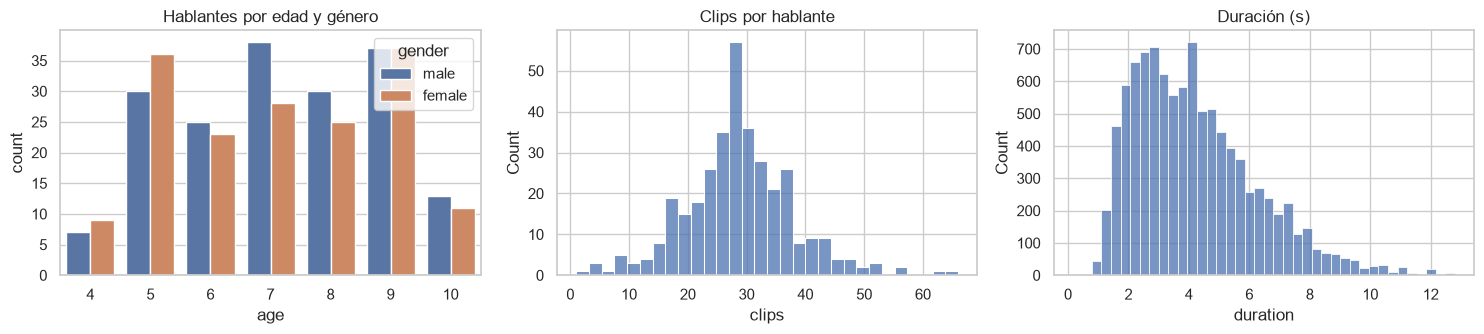
\includegraphics[width=\linewidth]{figuras/enni_hablantes_clips_duracion.png}
\caption{Corpus ENNI: hablantes por edad y género, fragmentos por hablante y duración de los fragmentos.}
\label{fig:enni}
\end{figure}

\begin{figure}[H]
\centering
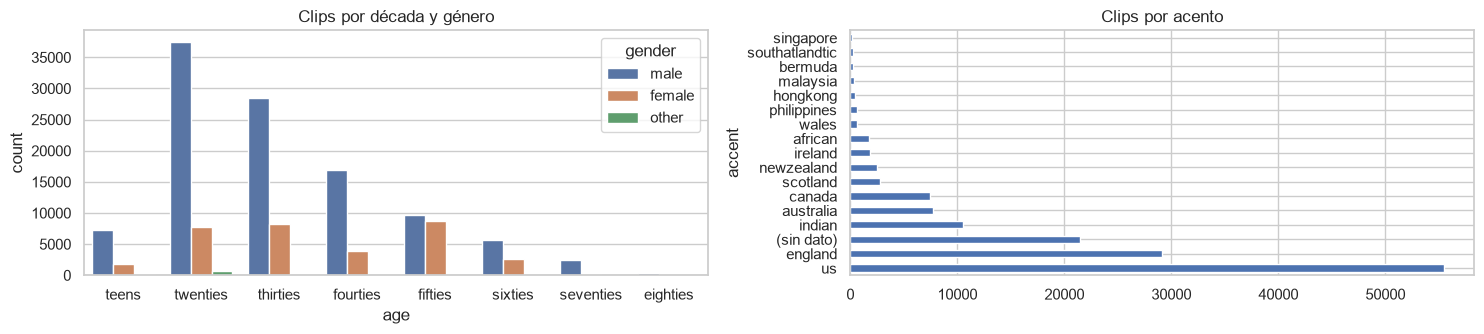
\includegraphics[width=\linewidth]{figuras/cv_clips_decada_acento.png}
\caption{Common Voice (fragmentos válidos con edad declarada): distribución por década de edad y género, y por acento. La década 10--19 corresponde a la etiqueta \emph{teens} del corpus.}
\label{fig:cv}
\end{figure}

El conjunto unido se construyó en cuatro pasos. Primero se descartaron los fragmentos marcados como inválidos en Common Voice, los de menos de $1\,\mathrm{s}$ o más de $15\,\mathrm{s}$ y los fragmentos mudos. Después, como esta versión de Common Voice no identifica a los hablantes, se agruparon sus fragmentos en \emph{pseudo-hablantes} por década, género y acento: una persona siempre declara los mismos datos, así que nunca queda repartida entre entrenamiento y prueba. En tercer lugar se limitaron los fragmentos por pseudo-hablante y se submuestreó a los adultos para equilibrar las clases. Por último, todo se convirtió a audio mono de $16\,\mathrm{kHz}$.

El resultado tiene \textbf{23\,893 fragmentos} y $27{,}7\,\mathrm{h}$ de audio: 9\,970 fragmentos de niños ($11{,}6\,\mathrm{h}$), 3\,960 de adolescentes ($4{,}1\,\mathrm{h}$) y 9\,963 de adultos ($12{,}0\,\mathrm{h}$). La figura~\ref{fig:corpus_clase} muestra que cada clase proviene de un solo corpus y que hay muy pocos grupos de adolescentes, y la figura~\ref{fig:dataset} resume el conjunto final. Las duraciones son parecidas entre clases (mediana cercana a $4\,\mathrm{s}$), pero los adolescentes son mayoritariamente hombres y su distribución de acentos difiere de la de los adultos, otra fuente posible de sesgo.

\begin{figure}[H]
\centering
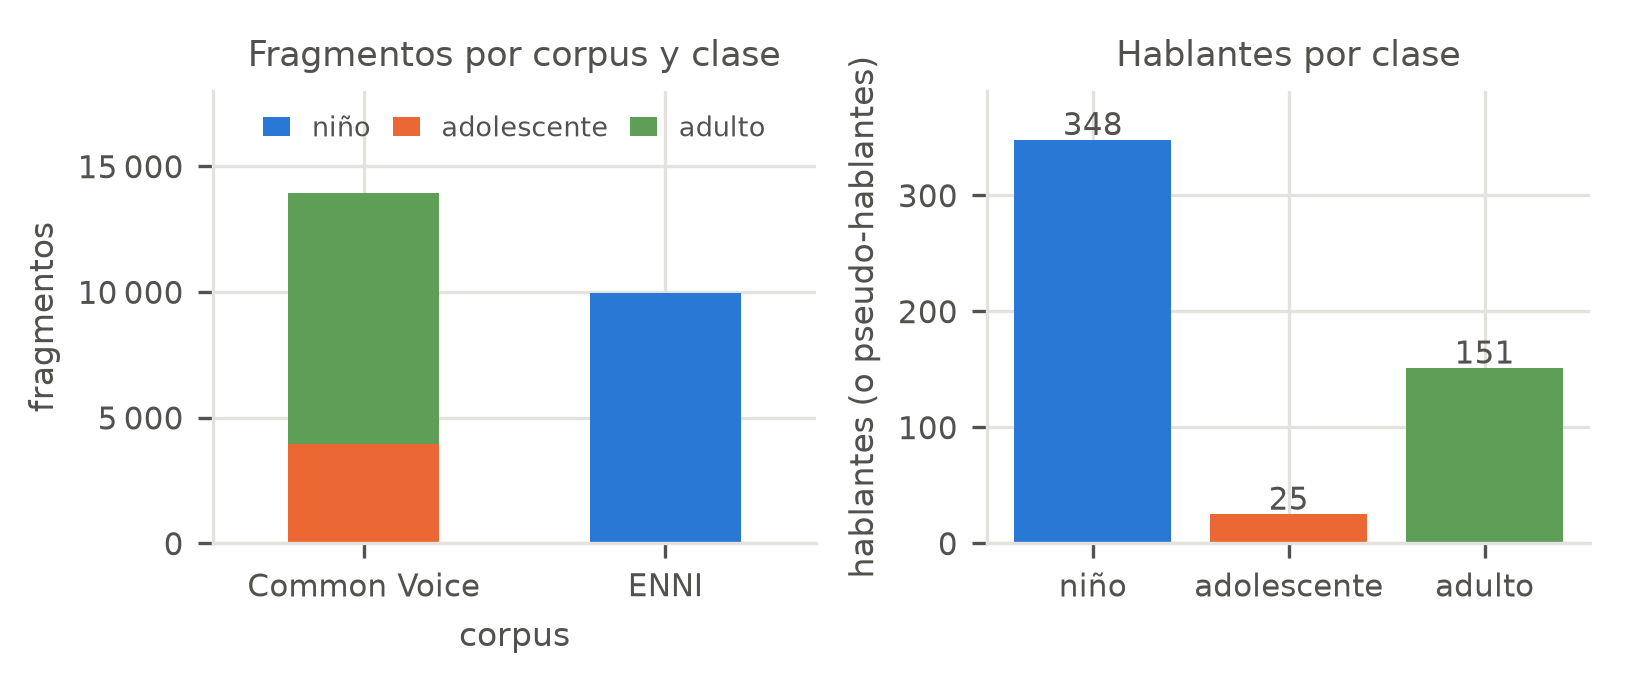
\includegraphics[width=0.85\linewidth]{figuras/clips_corpus_hablantes_clase.png}
\caption{Fragmentos por corpus y clase, y número de hablantes (o pseudo-hablantes) por clase en el conjunto unido.}
\label{fig:corpus_clase}
\end{figure}

\begin{figure}[H]
\centering
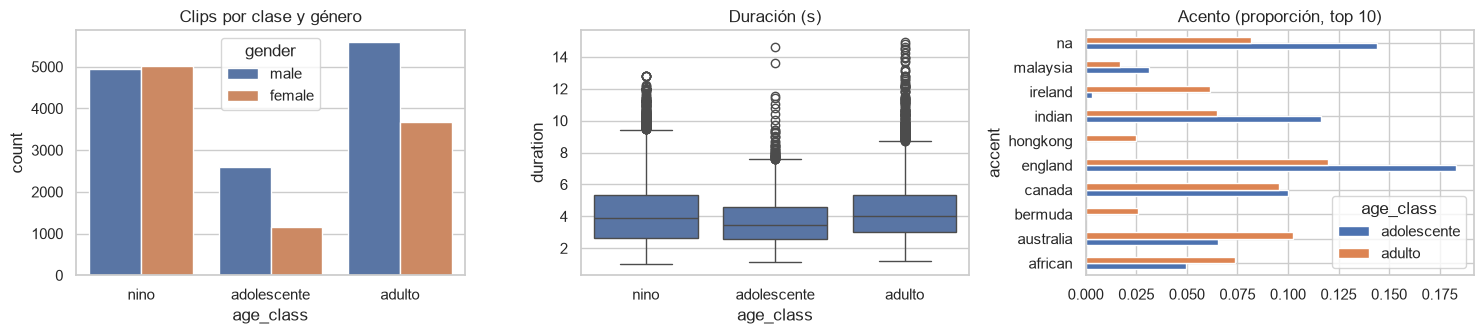
\includegraphics[width=\linewidth]{figuras/dataset_clase_duracion_acento.png}
\caption{Conjunto unido: fragmentos por clase y género, duración por clase (adol. = adolescente) y proporción de los diez acentos más frecuentes en adolescentes y adultos.}
\label{fig:dataset}
\end{figure}

Para evaluar con honestidad, la partición se hizo \textbf{por hablante}: ningún hablante aparece en dos particiones, porque si apareciera, el modelo memorizaría voces y las métricas saldrían infladas. Se repartieron hablantes completos en proporción aproximada 70/15/15 entre entrenamiento, validación y prueba (figura~\ref{fig:particiones}). En prueba quedaron 53 niños, 4 grupos de adolescentes y 24 grupos de adultos.

Como la voz depende del género (sección~\ref{sec:genero_teoria}), también se midió cómo se reparte en cada clase. La tabla~\ref{tab:genero_datos} muestra, para cada clase, el porcentaje de fragmentos de hombres, de mujeres y sin género declarado, y el número de hablantes de cada género en todo el conjunto y en prueba. En niños el género está equilibrado, pero en adolescentes casi dos de cada tres fragmentos son de hombres, y en prueba hay un único grupo de mujeres adolescentes. En adultos también predominan los hombres, y el 7\,\% de los fragmentos no declara género. Para Common Voice, cada ``hablante'' es un pseudo-hablante, así que estos conteos son una cota inferior del número real de personas.

\begin{table}[H]
\centering
\caption{Composición por género de cada clase: porcentaje de fragmentos y número de hablantes (H = hombres; M = mujeres).}
\label{tab:genero_datos}
\small
\begin{tabular}{@{}lccccccc@{}}
\toprule
& \multicolumn{3}{c}{\textbf{Fragmentos (\%)}} & \multicolumn{2}{c}{\textbf{Hablantes}} & \multicolumn{2}{c}{\textbf{Hablantes en prueba}} \\
\cmidrule(lr){2-4}\cmidrule(lr){5-6}\cmidrule(l){7-8}
\textbf{Clase} & \textbf{H} & \textbf{M} & \textbf{Sin dato} & \textbf{H} & \textbf{M} & \textbf{H} & \textbf{M} \\
\midrule
Niño        & 49,6 & 50,4 & 0,0 & 180 & 168 & 24 & 29 \\
Adolescente & 65,4 & 29,2 & 5,4 & 14  & 8   & 3  & 1 \\
Adulto      & 56,1 & 36,8 & 7,1 & 77  & 59  & 13 & 9 \\
\bottomrule
\end{tabular}
\end{table}

\begin{figure}[H]
\centering
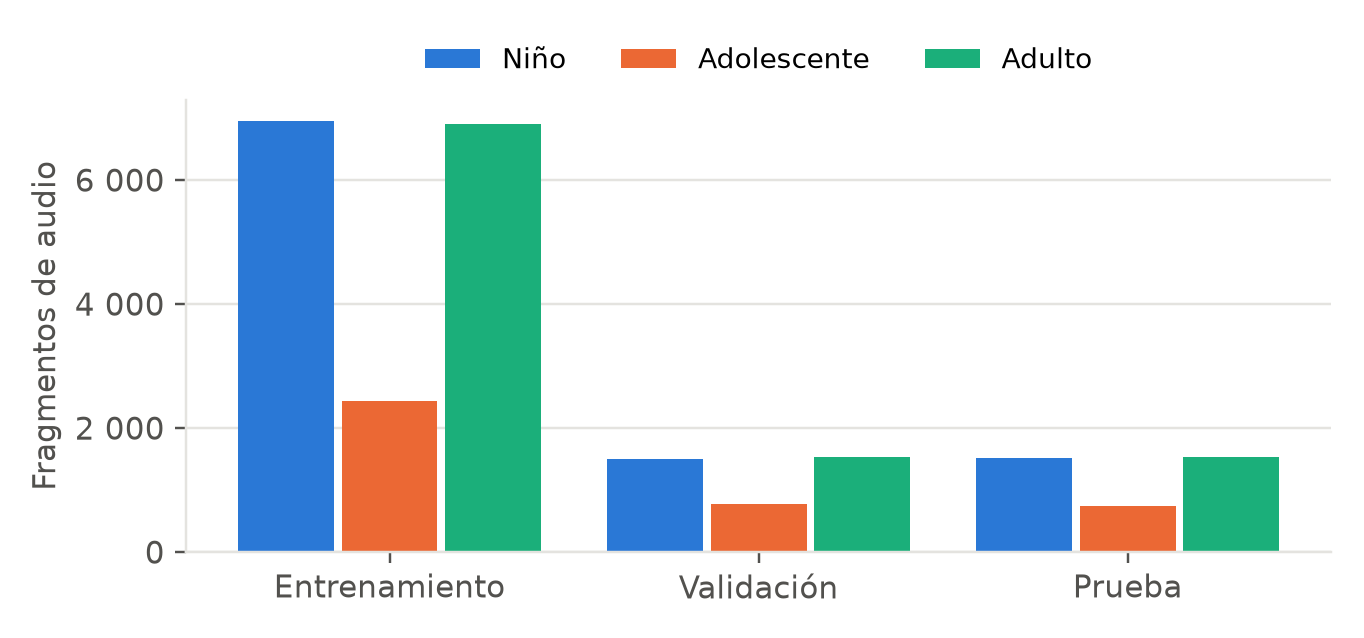
\includegraphics[width=0.7\linewidth]{figuras/particiones.png}
\caption{Fragmentos por clase en cada partición. La partición es por hablante: ninguna persona aparece en dos particiones.}
\label{fig:particiones}
\end{figure}

\subsection{Flujo del sistema}

La figura~\ref{fig:flujo} muestra el recorrido de un audio desde que entra al sistema hasta que llega a una persona revisora. El contenido de lo que se dice nunca se analiza.

\begin{figure}[H]
\centering
\begin{tikzpicture}[
  caja/.style={draw=tinta, fill=fondo, rounded corners=3pt, align=center, font=\footnotesize, minimum height=1.05cm, text width=2.7cm},
  flecha/.style={-{Stealth[length=2.2mm]}, thick, tinta}]
\node[caja] (a) {Audio de la\\conversación};
\node[caja, right=0.45cm of a] (b) {Detección de\\voz y diarización};
\node[caja, right=0.45cm of b] (c) {Edad por\\hablante};
\node[caja, right=0.45cm of c] (d) {Puntaje y\\nivel de riesgo};
\node[caja, below=0.7cm of d, fill=white] (e) {Revisión\\humana};
\node[caja, below=0.7cm of c, fill=white] (f) {Bandera de\\voz modificada};
\draw[flecha] (a) -- (b); \draw[flecha] (b) -- (c); \draw[flecha] (c) -- (d); \draw[flecha] (d) -- (e);
\draw[flecha] (c) -- (f); \draw[flecha] (f) -- (e);
\node[font=\scriptsize, text=tinta, below=0.08cm of b, text width=2.6cm, align=center] {¿quién habla\\y cuándo?};
\end{tikzpicture}
\caption{Flujo de punta a punta. La bandera de voz modificada es informativa: no altera el puntaje de riesgo.}
\label{fig:flujo}
\end{figure}

Los pasos son los siguientes:
\begin{enumerate}
  \item \textbf{Carga y normalización}: audio mono a $16\,\mathrm{kHz}$ con el volumen igualado, para que el modelo no aprenda que una fuente está grabada más fuerte que otra.
  \item \textbf{Detección de actividad de voz} por energía (todo lo que esté a más de 30\,dB por debajo del pico se considera silencio).
  \item \textbf{Diarización}: el habla se corta en ventanas de $1{,}5\,\mathrm{s}$ que avanzan cada $0{,}75\,\mathrm{s}$, a cada ventana se le calcula un vector ECAPA-TDNN y las ventanas se agrupan por similitud de coseno. Cada grupo es un hablante. Si se conoce el número de participantes, puede indicarse.
  \item \textbf{Estimación de edad}: el audio de cada hablante se divide en trozos de hasta $6\,\mathrm{s}$, el modelo estima las probabilidades de cada trozo y se promedian según su duración.
  \item \textbf{Bandera de voz modificada}: el detector de moduladores (sección~\ref{sec:metodo_moduladores}) estima, con el mismo vector ECAPA, si la voz de cada hablante pudo haber sido alterada.
  \item \textbf{Riesgo}: se combinan las probabilidades de todos los pares de hablantes (sección~\ref{sec:riesgo}).
\end{enumerate}

\subsection{Preprocesamiento y aumentación de datos}
\label{sec:filtros}

Antes de extraer características, cada fragmento se recorta a sus primeros $8\,\mathrm{s}$, se normaliza y se le quitan los silencios; los que quedan con menos de $1\,\mathrm{s}$ de voz se descartan. De los 23\,893 fragmentos quedaron 23\,560 válidos.

Para el entrenamiento, cada fragmento recibe además una \textbf{copia degradada} que imita la voz de un chat en un videojuego: un canal sucio más un fondo de partida. La tabla~\ref{tab:filtros} lista los doce filtros. Cada uno se aplica de forma independiente con la probabilidad indicada en la última columna, de modo que una copia puede recibir varios a la vez (en promedio, unos cinco), y al final se vuelve a normalizar el volumen. Los filtros cubren tres tipos de degradación: del canal (teléfono, reducción de bits, saturación, huecos, clics), de ruido (blanco, rosa, zumbido eléctrico, eco) y de fondo de partida (ambiente, música, efectos de juego). La aumentación se aplica por igual a todas las clases, para que ``audio ruidoso'' no se vuelva pista de clase, y \textbf{no se usa cambio de tono}, porque alteraría justo la señal de la edad; ninguno de los fondos contiene voces.

\begin{table}[H]
\centering
\caption{Filtros de aumentación. SNR = relación señal-ruido.}
\label{tab:filtros}
\small
\begin{tabularx}{\linewidth}{@{}>{\raggedright\arraybackslash}p{2.8cm}Lc@{}}
\toprule
\textbf{Filtro} & \textbf{Qué simula} & \textbf{Probabilidad} \\
\midrule
Teléfono & Banda de 300 a 3\,400\,Hz y paso por $8\,\mathrm{kHz}$ & 0,50 \\
Ruido blanco & Ruido de micrófono, SNR de 10 a 30\,dB & 0,70 \\
Saturación & Micrófono barato que recorta la señal & 0,30 \\
Ruido rosa & Ruido de ambiente más grave, SNR de 12 a 28\,dB & 0,40 \\
Huecos & Cortes de red: se silencia entre 2 y 8\,\% del audio & 0,30 \\
Zumbido & Zumbido eléctrico de 50 o 60\,Hz con su armónico & 0,25 \\
Clics & Chasquidos sueltos & 0,25 \\
Eco & Una reflexión con retardo de $60$ a $180\,\mathrm{ms}$ & 0,30 \\
Reducción de bits & Códec de chat de baja calidad (5 a 8 bits) & 0,25 \\
Ambiente & Ruido de fondo grave o ventilador de computadora, SNR de 8 a 22\,dB & 0,50 \\
Música de fondo & Acorde sostenido sintético, SNR de 8 a 20\,dB & 0,50 \\
Efectos de juego & Pasos o disparos rítmicos y pitidos de interfaz & 0,40 \\
\bottomrule
\end{tabularx}
\end{table}

Para entender qué le hace cada filtro a la señal de edad, se midieron el tono, los formantes y varios rasgos espectrales de un fragmento de cada clase, limpio y con cada filtro por separado. Se observaron tres efectos. El \textbf{canal telefónico borra los formantes altos}: en el niño de ejemplo, $F_2$ baja de 2\,428 a 1\,379\,Hz y $F_3$ de 3\,798 a 2\,398\,Hz, justo las resonancias que delatan un tracto vocal corto, y en el adulto provocó además un error de octava en el estimador de tono (de 142 a 291\,Hz). El \textbf{ruido y la reducción de bits inventan formantes}: en el adulto de ejemplo, $F_1$ sube de 346\,Hz a más de 1\,000\,Hz con ruido blanco, ruido rosa o reducción de bits, porque el análisis confunde picos de ruido con resonancias, y un adulto ``parece'' tener el tracto de un niño. Por último, \textbf{el tono casi no se mueve}: fuera del error de octava, cambia menos de 20\,Hz con cualquier filtro. Los riesgos están en los formantes y el timbre, no en el tono.

La figura~\ref{fig:mfcc} muestra ese efecto sobre los MFCC del mismo fragmento adulto. El canal telefónico cambia sobre todo los primeros coeficientes, que describen la inclinación general del espectro: al cortar las frecuencias graves y agudas aparecen franjas oscuras en los coeficientes 2 a 4. El ruido blanco borra el contraste entre los momentos de voz y las pausas, porque el ruido llena también los silencios. La música de fondo, en cambio, deja el patrón casi intacto. Por eso se entrena con estas copias degradadas: para que los modelos aprendan a reconocer la edad a pesar de esos cambios.

\begin{figure}[H]
\centering
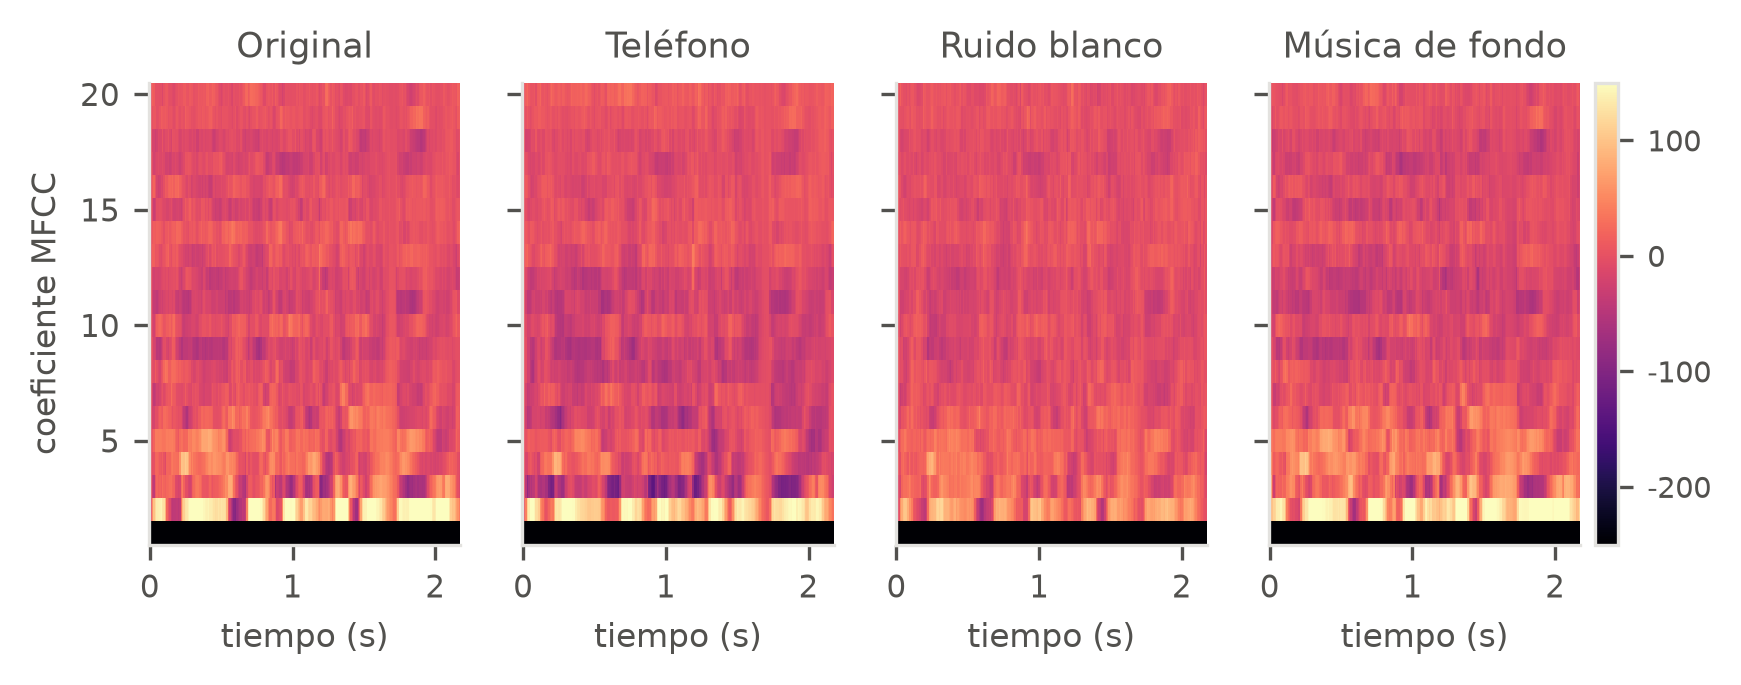
\includegraphics[width=0.91\linewidth]{figuras/mfcc_filtros.png}
\caption{MFCC (20 coeficientes, un cuadro cada $10\,\mathrm{ms}$) del fragmento adulto de ejemplo, limpio y con tres de los doce filtros. El color indica el valor de cada coeficiente; la franja inferior es el coeficiente 1, que mide la energía total.}
\label{fig:mfcc}
\end{figure}

\subsection{Extracción de características}
\label{sec:extraccion}

Cada fragmento se convierte en un vector numérico de longitud fija con tres extractores distintos, que la tabla~\ref{tab:extractores} compara. El extractor acústico clásico es el único interpretable rasgo por rasgo: combina el logaritmo del tono (5 estadísticos), los tres primeros formantes estimados por predicción lineal (15), los MFCC con sus deltas (80, sección~\ref{sec:mfcc}), cinco rasgos espectrales con su media y desviación (10), el contraste espectral (7) y la proporción de cuadros con voz (1). Los dos extractores neuronales usan modelos preentrenados congelados: ECAPA-TDNN produce un vector de 192 dimensiones y de WavLM se toman la media y la desviación estándar en el tiempo del promedio de las capas 3 a 8. La última columna muestra el costo de cada extractor en CPU, que domina el tiempo de inferencia.

\begin{table}[H]
\centering
\caption{Extractores de características.}
\label{tab:extractores}
\small
\begin{tabularx}{\linewidth}{@{}>{\raggedright\arraybackslash}p{2.9cm}cLc@{}}
\toprule
\textbf{Extractor} & \textbf{Dimensiones} & \textbf{Qué representa} & \textbf{Tiempo ($\mathrm{ms}$)} \\
\midrule
Acústico clásico & 118 & Tono, formantes $F_1$ a $F_3$, MFCC con deltas y rasgos espectrales & $17$ \\
ECAPA-TDNN~\cite{ecapa2020} & 192 & ``Huella vocal'' de una red entrenada para reconocer hablantes (SpeechBrain~\cite{speechbrain2021}, VoxCeleb) & $30$ \\
WavLM-base-plus~\cite{wavlm2022} & 1\,536 & Media y desviación estándar de las capas 3 a 8 del modelo autosupervisado & $87$ \\
\bottomrule
\end{tabularx}
\end{table}

La figura~\ref{fig:f0} confirma en nuestros datos lo que predice el marco teórico, usando la primera característica del vector acústico: los niños tienen un tono claramente más alto (mediana de 242\,Hz), mientras que los adolescentes y los adultos se superponen casi por completo (147 y 154\,Hz).

\begin{figure}[H]
\centering
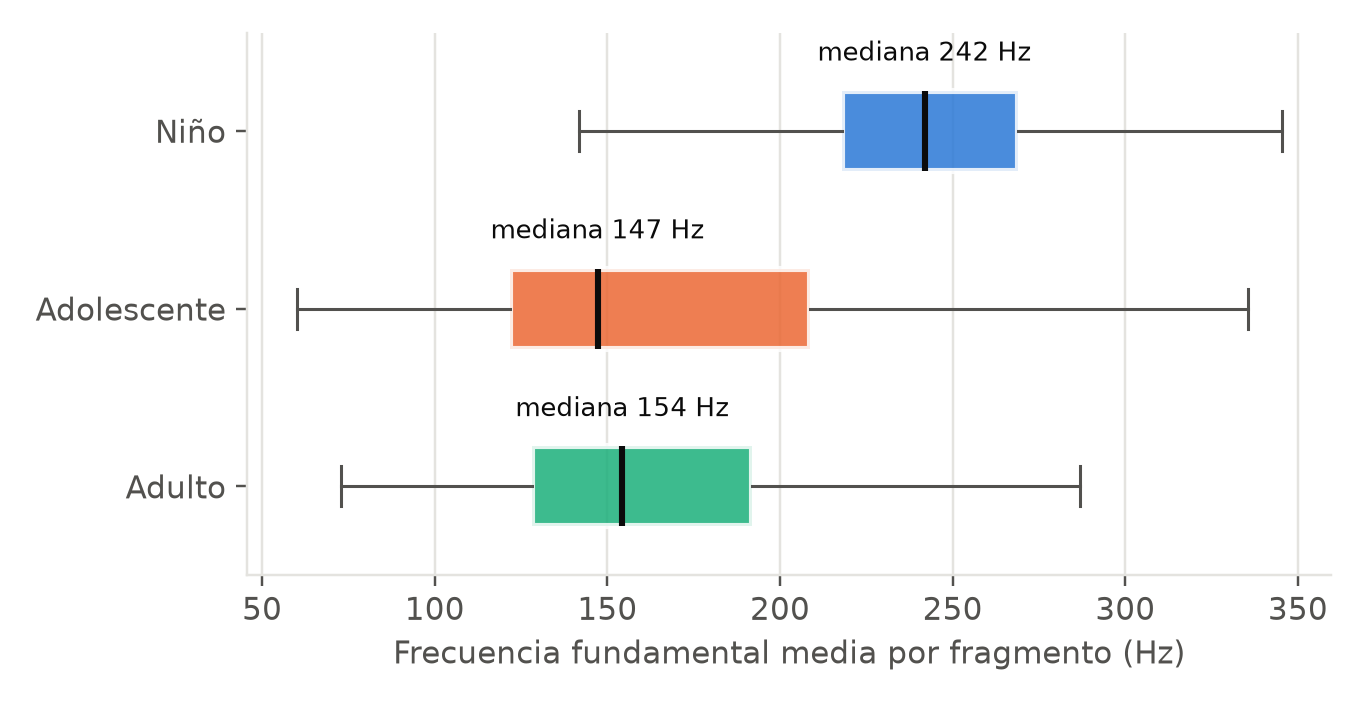
\includegraphics[width=0.62\linewidth]{figuras/f0_por_clase.png}
\caption{Tono fundamental medio de cada fragmento, por clase de edad, en todo el conjunto de datos.}
\label{fig:f0}
\end{figure}

\subsection{Modelos comparados}

Se entrenaron seis modelos, cada uno formado por una representación y un clasificador, que la tabla~\ref{tab:modelos} justifica uno por uno. Los tres principales (A, B, C) cubren de la representación más interpretable a la más potente. Los otros tres son variantes que permiten separar qué aporta la representación y qué aporta el clasificador: A2 y A3 cambian el clasificador de A, y B2 el de B. La segunda columna de clasificadores indica si el modelo es paramétrico o no (sección~\ref{sec:clasificadores}).

\begin{table}[H]
\centering
\caption{Modelos comparados y justificación. P = paramétrico; NP = no paramétrico.}
\label{tab:modelos}
\small
\begin{tabularx}{\linewidth}{@{}l>{\raggedright\arraybackslash}p{2.75cm}>{\raggedright\arraybackslash}p{2.5cm}cL@{}}
\toprule
& \textbf{Representación} & \textbf{Clasificador} & \textbf{Tipo} & \textbf{Por qué} \\
\midrule
A & Acústica clásica & Potenciación del gradiente~\cite{sklearn2011} & NP & La fisiología explica la edad. Los árboles capturan umbrales no lineales (``tono alto y formantes altos $\Rightarrow$ niño''), son interpretables y corren en cualquier computadora. \\
B & ECAPA-TDNN & SVM con núcleo radial & NP & ECAPA es el estado del arte en reconocimiento de hablante; su vector resume tamaño del tracto vocal, timbre y tono. Es compacto, y la SVM generaliza bien con pocos datos de menores gracias al margen máximo. Además, el mismo vector sirve para la diarización. \\
C & WavLM & Regresión logística & P & Un clasificador lineal sobre el modelo congelado evita el sobreajuste con pocos datos y permite entrenar en una computadora personal. \\
A2 & Acústica clásica & Bosque aleatorio & NP & Línea base liviana sin redes neuronales; ¿aporta la potenciación frente a árboles independientes? \\
A3 & Acústica clásica & Regresión logística & P & Piso de referencia: ¿basta un modelo lineal sobre rasgos fisiológicos? \\
B2 & ECAPA-TDNN & Bosque aleatorio & NP & Misma representación que B con otro clasificador. \\
\bottomrule
\end{tabularx}
\end{table}

\subsection{Protocolo de entrenamiento}

Para que la comparación sea justa, todos los modelos siguen el mismo protocolo:
\begin{itemize}
  \item \textbf{Pesos de clase balanceados}, porque hay menos adolescentes.
  \item \textbf{Entrenamiento con aumentación}: cada fragmento de entrenamiento aparece limpio y con su copia degradada.
  \item \textbf{Hiperparámetros} elegidos con una búsqueda en cuadrícula sobre el conjunto de validación, usando F1-macro.
  \item \textbf{Calibración sigmoide} sobre validación.
  \item \textbf{Evaluación una sola vez} en el conjunto de prueba, con hablantes que el modelo nunca vio.
  \item \textbf{Selección} del ganador por F1-macro en prueba; si dos modelos quedan a menos de 0,01, gana el de mayor sensibilidad para niños.
\end{itemize}

\subsection{Detector de moduladores de voz}
\label{sec:metodo_moduladores}

Un adulto que usa un modulador para sonar más joven puede engañar al modelo de edad: si el sistema oye ``dos niños'' en lugar de ``niño + adulto'', el riesgo baja. Para mitigarlo se entrenó un detector binario ---¿esta voz pasó por un modulador?--- que funciona como \textbf{bandera informativa} junto al puntaje: no cambia la fórmula del riesgo ni las probabilidades de edad, solo avisa que la edad estimada de ese hablante es menos fiable y conviene priorizar su revisión.

Los datos del detector se construyeron sin modificar el conjunto original. A una cuarta parte de los fragmentos adultos de cada partición se le generó una copia modulada ---2\,446 copias en total, sin fallos--- y los originales se conservaron; cada copia hereda el hablante y la partición del original, así que no hay fuga entre entrenamiento y prueba. La intensidad se sorteó con un solo factor de tono entre 1,2 y 1,8 (de 3 a 10 semitonos), con los formantes movidos por su raíz cuadrada; el 75\,\% de las copias sube el tono y el 25\,\% lo baja, para que el detector no aprenda simplemente ``voz aguda = modulada'' y no marque a los niños reales. Entrenamiento y validación usan solo el cambio de tono simple y Praat; el vocoder WORLD \textbf{aparece solo en prueba}, para medir si el detector reconoce un modulador que nunca vio. Los negativos son todos los fragmentos originales de las tres clases, de modo que solo el 9,4\,\% de los fragmentos está modulado.

El detector es una cabeza sobre el mismo vector ECAPA de 192 dimensiones que ya usan la diarización y el modelo de edad, así que no añade costo de extracción. Se compararon una SVM (no paramétrica) y una regresión logística (paramétrica) con el mismo protocolo de los modelos de edad. Como la clase modulada es rara, los hiperparámetros se eligieron por precisión media en validación, y el umbral de decisión se fijó también en validación, maximizando el F1 de la clase ``modulado''.

Se entrenaron dos versiones del detector. La primera, el \textbf{detector limpio}, solo ve audio sin degradar. En un chat de voz real, sin embargo, el modulador actúa en la fuente y después el canal degrada la señal, así que la segunda versión, el \textbf{detector acoplado}, respeta ese orden: cada copia modulada pasa \emph{después} por los mismos doce filtros de la tabla~\ref{tab:filtros}. La regla clave es el \textbf{mismo trato para ambos grupos}: cada fragmento, original o modulado, recibe una copia con canal con las mismas probabilidades por filtro, porque si solo se degradara un grupo, el detector aprendería el atajo ``audio sucio = modulado''. El detector acoplado se entrena con las versiones limpia y con canal de todos los fragmentos (52\,002 en total), para que funcione en ambas condiciones.

\subsection{Puntaje de riesgo}
\label{sec:riesgo}

El puntaje responde a una sola pregunta: ¿qué tan seguros estamos de que en este audio hablan una persona menor de edad y una persona adulta distintas? Para cada par de hablantes distintos $i$ (posible menor) y $j$ (posible adulto) se calcula
\begin{equation}
r(i,j) = P_i(\text{niño})\,P_j(\text{adulto}) \cdot 0{,}90 \;+\; P_i(\text{adolescente})\,P_j(\text{adulto}) \cdot 0{,}60.
\end{equation}
El riesgo del audio es el máximo sobre todos los pares, porque basta una pareja menor--adulto para alertar, con un piso de 0,05 para no afirmar nunca ``riesgo cero''. Los niveles son \textbf{bajo} ($<0{,}30$), \textbf{medio} ($0{,}30$ a $0{,}60$) y \textbf{alto} ($\geq 0{,}60$). Los pesos (0,90 y 0,60) reflejan que la pareja niño--adulto es la de mayor preocupación y que la etiqueta de adolescente es menos fiable; ambos son menores que 1 porque, aun con certeza total sobre las edades, la combinación no prueba un abuso. Por ejemplo, si un hablante es niño con 95\,\% de probabilidad y otro adulto con 90\,\%, el riesgo es $0{,}95 \times 0{,}90 \times 0{,}90 \approx 0{,}77$. Si el modelo duda, el riesgo baja en proporción.

\subsection{Implementación y despliegue}

El sistema está escrito en Python como un paquete compartido por el cuaderno de entrenamiento y el servicio. El modelo ganador y el detector de moduladores se sirven mediante una API web (FastAPI) en un contenedor Docker que funciona sin conexión a internet y solo con CPU. La ruta \texttt{/analyze} recibe un archivo de audio de hasta $10\,\mathrm{min}$ y devuelve el puntaje de riesgo (0 a 1), su nivel, el número de hablantes detectados y, para cada uno, su duración, sus intervalos de habla, sus probabilidades de edad y la bandera de voz modificada (su probabilidad, el umbral y si lo supera). Todas las respuestas incluyen un \textbf{aviso obligatorio} de que el resultado es una alerta y no un veredicto. El audio se procesa en un archivo temporal que se borra al terminar: el servicio no conserva grabaciones ni transcripciones.

%=====================================================================
\section{Resultados}
%=====================================================================

Los resultados se presentan en el mismo orden que la metodología: primero la comparación de los modelos de edad y su eficiencia, después la auditoría de sesgo por canal, el sistema completo con conversaciones simuladas, el detector de moduladores y, por último, las pruebas del sistema.

\subsection{Comparativa de modelos}

La tabla~\ref{tab:resultados} compara los seis modelos en el conjunto de prueba, con 3\,724 fragmentos de hablantes nunca vistos; cada fila es un modelo y cada columna una de las métricas de la sección~\ref{sec:metricas}. El modelo B (ECAPA-TDNN + SVM, con $C = 0{,}3$) obtuvo el mejor F1-macro, la mejor exactitud balanceada, la mejor sensibilidad para adolescentes y el mejor AUC, y es el que usa el sistema. La figura~\ref{fig:modelos} resume las dos columnas que más los separan.

\begin{table}[H]
\centering
\caption{Resultados en el conjunto de prueba (por fragmento). En negritas, el mejor valor de cada columna.}
\label{tab:resultados}
\footnotesize
\setlength{\tabcolsep}{4pt}
\begin{tabular}{@{}lcccccc@{}}
\toprule
\textbf{Modelo} & \textbf{F1-macro} & \textbf{Exact. bal.} & \textbf{Sens. niño} & \textbf{Sens. adol.} & \textbf{Sens. adulto} & \textbf{AUC} \\
\midrule
B ECAPA + SVM          & \textbf{0,812} & \textbf{0,809} & 0,986 & \textbf{0,590} & 0,850 & \textbf{0,944} \\
C WavLM + reg. log.    & 0,784 & 0,775 & \textbf{0,999} & 0,409 & 0,918 & 0,941 \\
B2 ECAPA + bosque      & 0,776 & 0,768 & 0,963 & 0,428 & 0,912 & \textbf{0,944} \\
A2 Acústico + bosque   & 0,731 & 0,730 & 0,995 & 0,302 & 0,894 & 0,902 \\
A Acústico + pot. grad.& 0,691 & 0,699 & 0,997 & 0,213 & 0,886 & 0,877 \\
A3 Acústico + reg. log.& 0,590 & 0,652 & 0,997 & 0,003 & \textbf{0,956} & 0,870 \\
\bottomrule
\end{tabular}

\vspace{2pt}
{\footnotesize Sens. = sensibilidad. AUC = área bajo la curva ROC para separar menores de adultos.}
\end{table}

\begin{figure}[H]
\centering
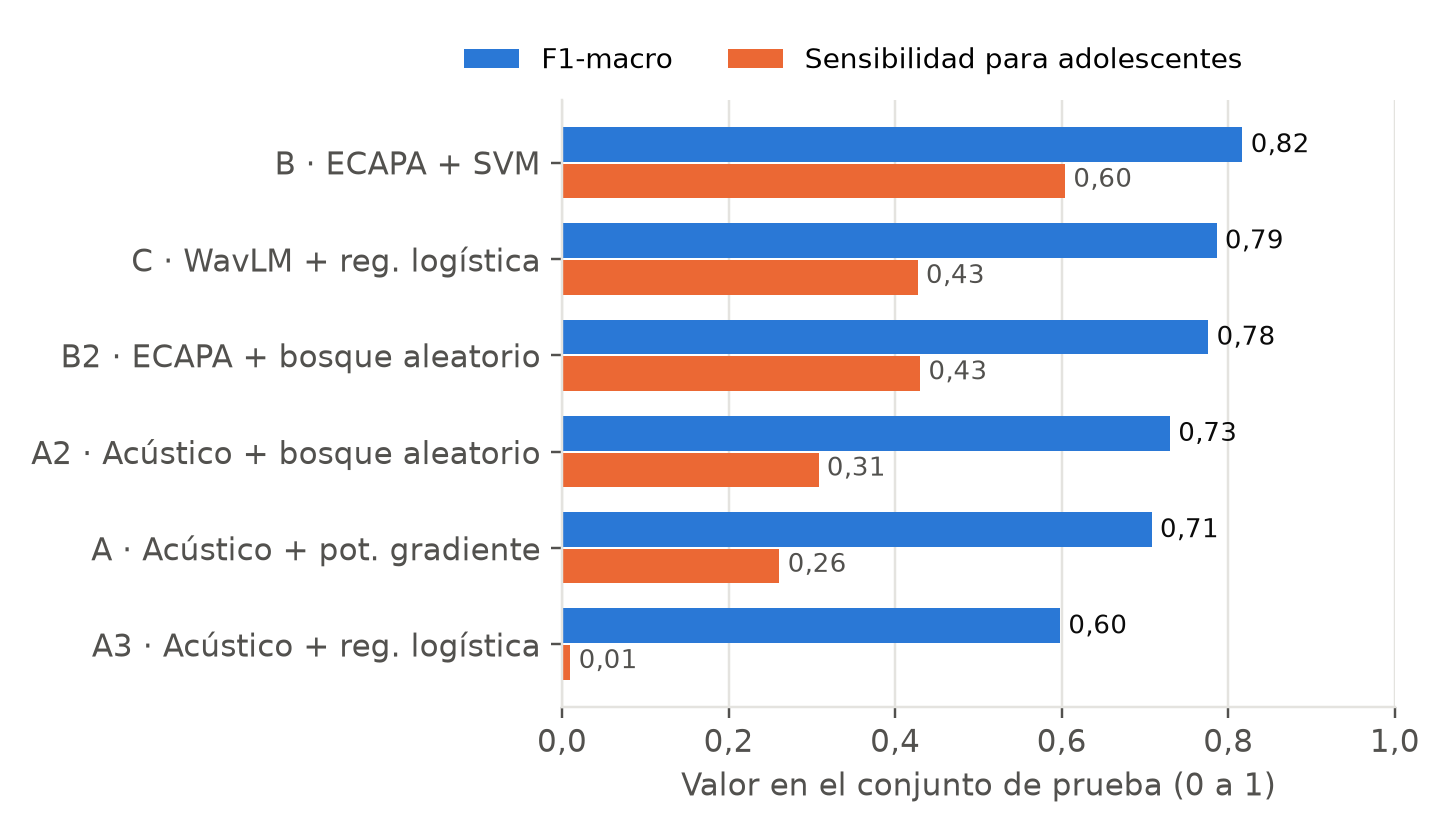
\includegraphics[width=0.85\linewidth]{figuras/comparativa_modelos.png}
\caption{F1-macro y sensibilidad para adolescentes de cada modelo en el conjunto de prueba.}
\label{fig:modelos}
\end{figure}

De la tabla se desprenden varias lecturas. La primera es que \textbf{la representación pesa más que el clasificador}: con rasgos acústicos el mejor modelo llega a 0,731 de F1-macro, mientras que con ECAPA incluso un bosque aleatorio sube a 0,776. Con la misma representación ECAPA, la SVM supera al bosque aleatorio (0,812 frente a 0,776), y la diferencia está en los adolescentes (0,590 frente a 0,428). En el otro extremo, el modelo lineal sobre rasgos acústicos (A3) prácticamente no detecta adolescentes (0,003): como muestra la figura~\ref{fig:f0}, su tono es casi igual al de los adultos, y la frontera entre ambas clases no es lineal en esos rasgos. Esto favorece a los clasificadores no paramétricos: los dos mejores modelos sobre un mismo extractor son siempre no paramétricos (B sobre ECAPA, A2 sobre rasgos acústicos), y el único paramétrico competitivo es C, que compensa con la representación más rica.

En validación, WavLM superaba a ECAPA (0,763 frente a 0,739 de F1-macro), pero en prueba ECAPA lo supera por 0,028. Con tan pocos grupos de adolescentes (7 en validación y 4 en prueba), el orden entre los dos mejores modelos es sensible a qué hablantes caen en cada partición. Respecto a una versión anterior del proyecto, entrenada con solo tres filtros de aumentación, el F1-macro de todos los modelos cambia menos de 0,02; los nueve filtros nuevos casi no costaron rendimiento con audio limpio.

La figura~\ref{fig:confusion} muestra las matrices de confusión normalizadas por clase real. El error típico del modelo B es confundir adolescentes con adultos (el 40\,\% de los fragmentos adolescentes se clasifican como adultos); casi nunca confunde a un niño con un adulto. La sensibilidad para niños (0,96 a 1,00 en todos los modelos) debe leerse con cautela, porque todos los niños provienen de habla sintetizada (sección~\ref{sec:sesgo}).

\begin{figure}[H]
\centering
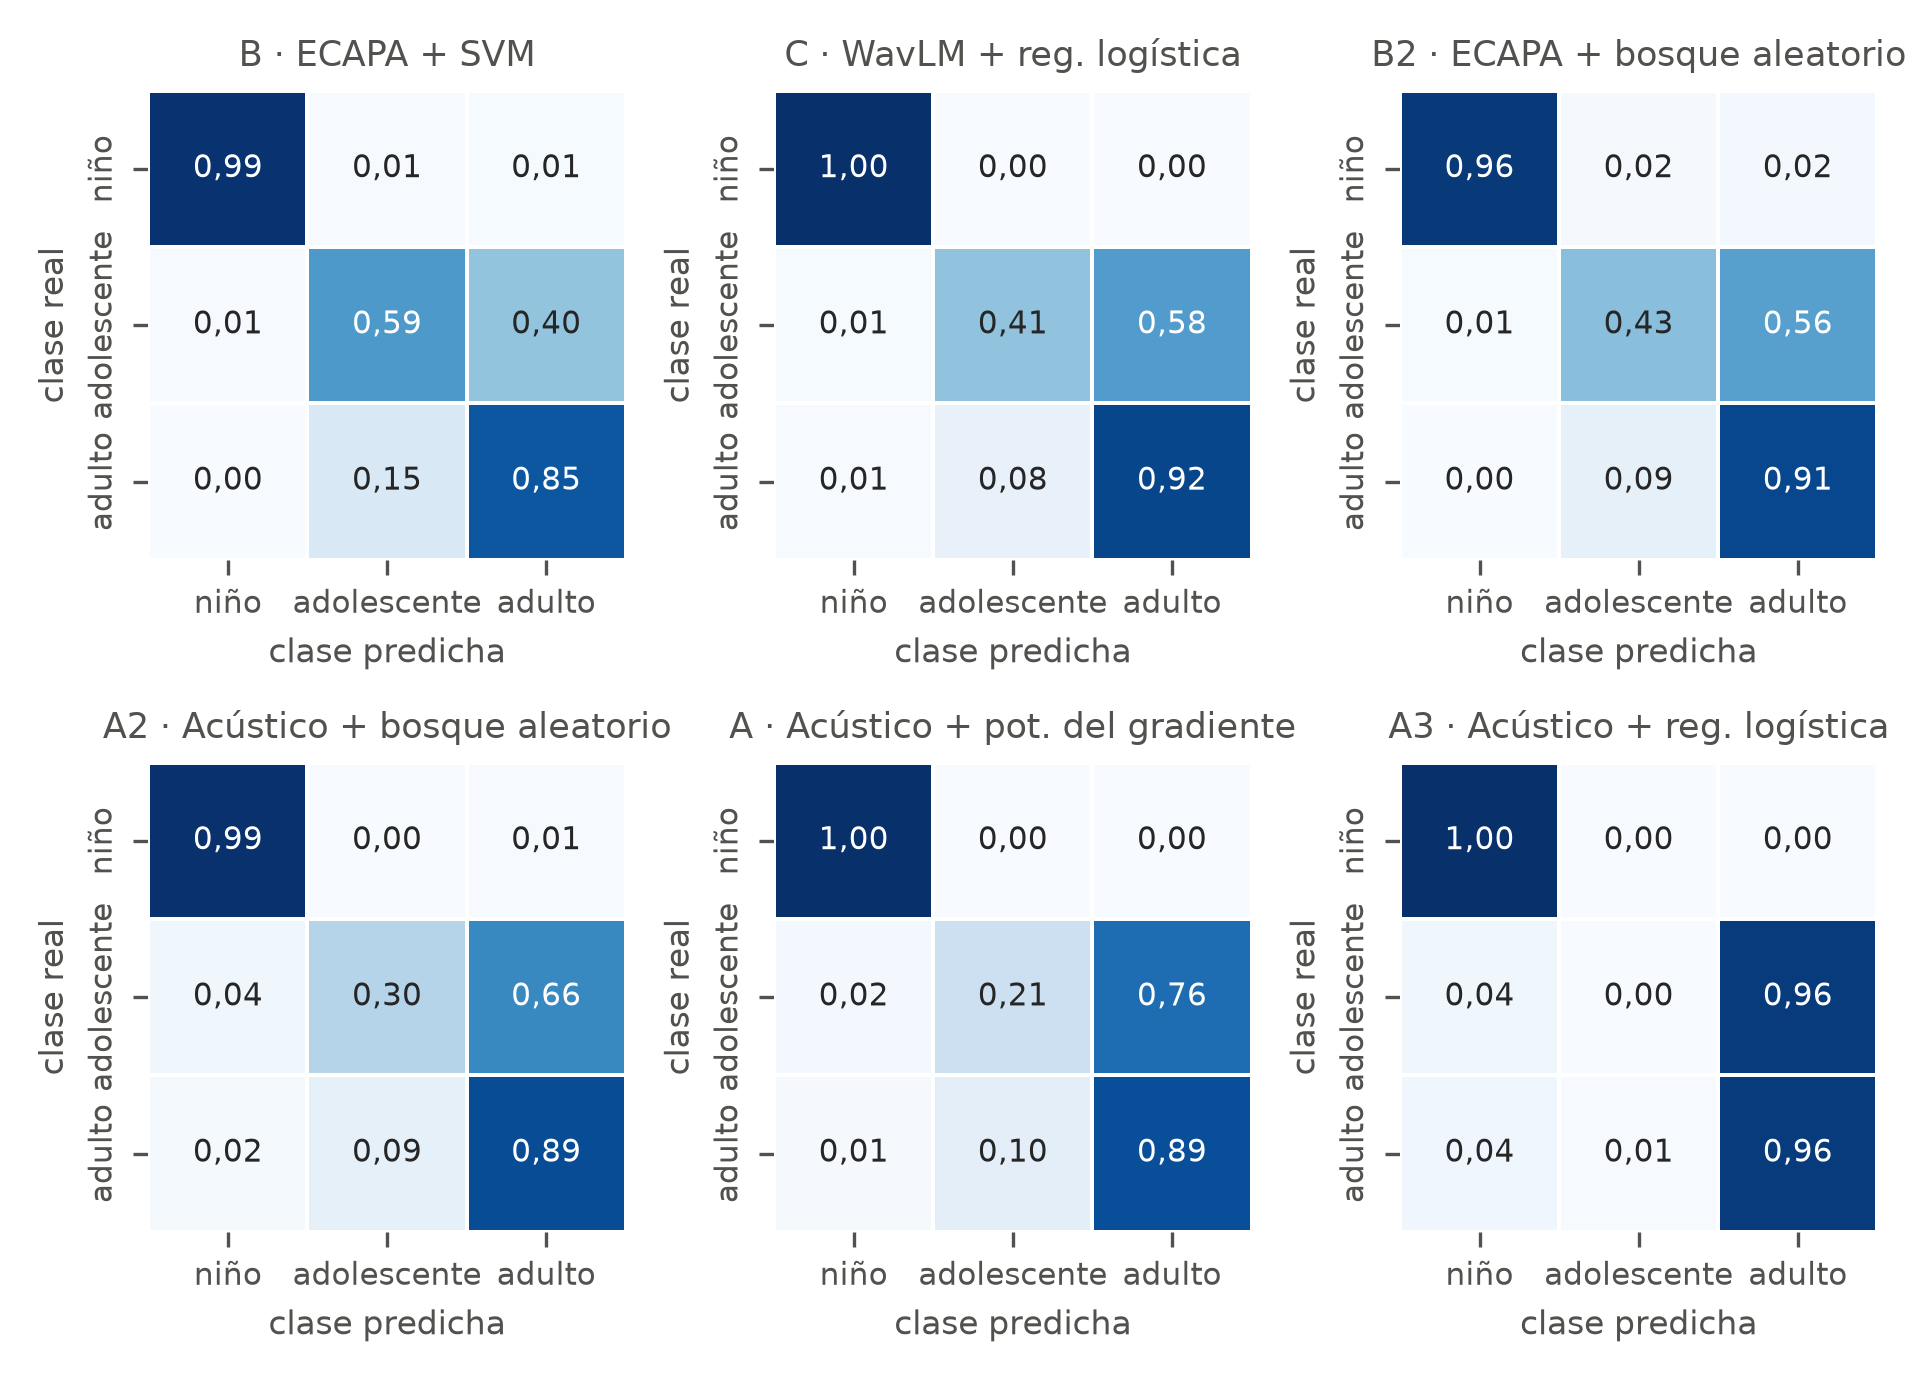
\includegraphics[width=\linewidth]{figuras/matrices_confusion.png}
\caption{Matrices de confusión normalizadas por clase real (filas) en el conjunto de prueba, para los seis modelos. La diagonal es la sensibilidad de cada clase.}
\label{fig:confusion}
\end{figure}

Al nivel de hablante, promediando las predicciones de todos los fragmentos de cada persona, el modelo B alcanza un F1-macro de 0,837, una exactitud balanceada de 0,819 y un AUC de 0,996; detecta al 100\,\% de los niños y al 95,8\,\% de los adultos. Su sensibilidad para adolescentes es de 0,50, pero se calcula sobre solo 4 grupos de adolescentes en prueba, por lo que es muy imprecisa.

\subsection{Eficiencia}

El costo de inferencia lo pone casi por completo el extractor, no el clasificador. La tabla~\ref{tab:eficiencia} compara, para los tres modelos más relevantes, el tiempo por fragmento en CPU y el tamaño en disco del clasificador y de la red preentrenada.

\begin{table}[H]
\centering
\caption{Tiempo de inferencia por fragmento en CPU y tamaño en disco.}
\label{tab:eficiencia}
\small
\begin{tabular}{@{}lcccc@{}}
\toprule
\textbf{Modelo} & \textbf{F1-macro} & \textbf{Tiempo ($\mathrm{ms}$)} & \textbf{Clasificador (MB)} & \textbf{Red (MB)} \\
\midrule
B ECAPA + SVM         & 0,812 & $31$ & 17,0 & 83 \\
C WavLM + reg. log.   & 0,784 & $87$ & 0,1 & 378 \\
A2 Acústico + bosque  & 0,731 & $17$ & 39,3 & 0 \\
\bottomrule
\end{tabular}
\end{table}

El modelo A2 es la mejor opción sin redes neuronales y tarda casi la mitad que B. Pero el sistema necesita ECAPA de todos modos para la diarización y el detector de moduladores, así que cambiar a A2 casi no ahorraría recursos y costaría 0,08 de F1-macro y la mitad de la sensibilidad para adolescentes. Ya desplegado, tras la carga inicial del modelo, analizar una conversación de $10\,\mathrm{s}$ toma menos de $0{,}2\,\mathrm{s}$.

\subsection{Auditoría de sesgo por canal}
\label{sec:sesgo}

El mayor riesgo metodológico es que \textbf{clase y fuente coinciden}: todos los niños vienen de habla sintetizada y limpia, y todos los demás de grabaciones caseras. El modelo podría aprender ``qué tipo de audio es'' en lugar de ``qué edad tiene''. Se hicieron tres comprobaciones.

La primera midió las diferencias de canal (figura~\ref{fig:canal}). Antes de normalizar, los audios infantiles eran unos 13\,dB más bajos y tenían otro espectro. La diferencia de volumen se elimina con la normalización; la de espectro, no. La segunda midió la predictibilidad de la fuente: un clasificador simple adivina el corpus de origen en el 98,8\,\% de los casos con los vectores ECAPA, frente a 57,9\,\% por azar. Con estos datos es inevitable, porque predecir la fuente equivale a predecir ``niño''.

\begin{figure}[H]
\centering
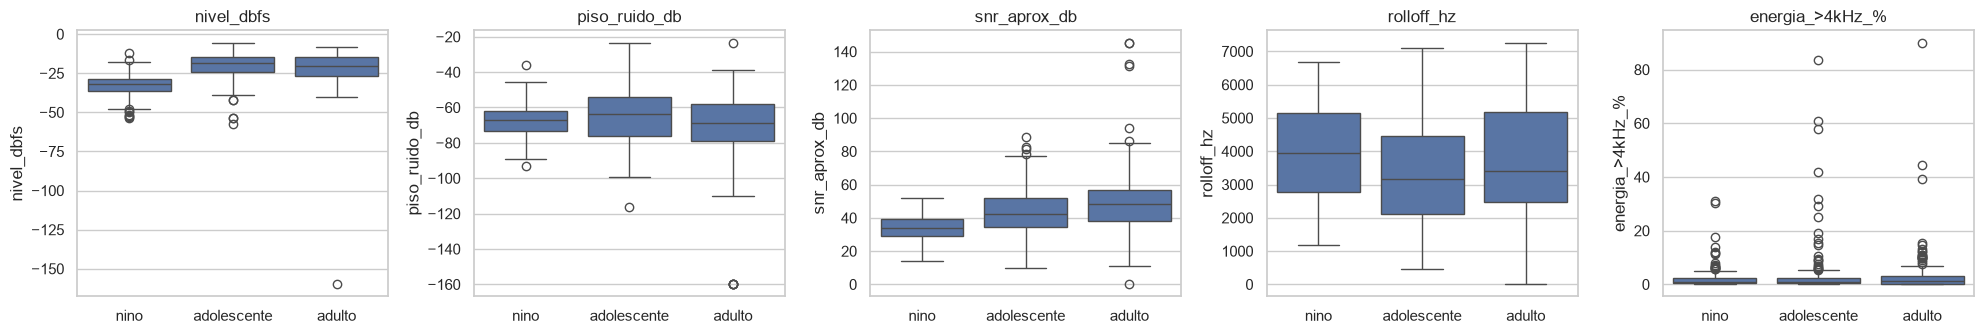
\includegraphics[width=\linewidth]{figuras/dataset_canal_por_clase.png}
\caption{Rasgos de canal por clase, en una muestra de 150 fragmentos por clase antes de normalizar: nivel, piso de ruido, relación señal-ruido aproximada, frecuencia bajo la que queda el 99\,\% de la energía y porcentaje de energía por encima de $4\,\mathrm{kHz}$. Las cajas muestran el rango intercuartil y la línea, la mediana.}
\label{fig:canal}
\end{figure}

La tercera comprobación, la robustez al canal, degradó todo el audio de prueba con la misma combinación aleatoria de los doce filtros. Si el modelo usara ``audio limpio = niño'', su sensibilidad para niños se desplomaría. La tabla~\ref{tab:robustez} compara el modelo B con el audio de prueba original y degradado: la caída es pequeña (0,019 de F1-macro) y la sensibilidad para niños baja solo dos puntos, aunque la degradación es mucho más dura que en la versión anterior del proyecto, que solo usaba canal telefónico, ruido blanco y saturación. Lo que más se pierde es la sensibilidad para adolescentes, que pasa de 0,590 a 0,551. El modelo no depende de que el audio sea limpio, pero todavía podría apoyarse en que la voz infantil es sintetizada; descartarlo exige un corpus con niños y adultos reales grabados en las mismas condiciones.

\begin{table}[H]
\centering
\caption{Modelo B con audio de prueba original y degradado con los doce filtros.}
\label{tab:robustez}
\small
\begin{tabular}{@{}lccccc@{}}
\toprule
\textbf{Audio} & \textbf{F1-macro} & \textbf{Sens. niño} & \textbf{Sens. adol.} & \textbf{Sens. adulto} & \textbf{AUC} \\
\midrule
Original  & 0,812 & 0,986 & 0,590 & 0,850 & 0,944 \\
Degradado & 0,793 & 0,966 & 0,551 & 0,851 & 0,939 \\
\bottomrule
\end{tabular}
\end{table}

\subsection{Análisis por género}
\label{sec:genero}

El desbalance de género de la tabla~\ref{tab:genero_datos} y las diferencias fisiológicas de la sección~\ref{sec:genero_teoria} obligan a revisar si el sistema trata igual a hombres y mujeres. El análisis se hizo en tres niveles: la acústica de los datos, el modelo de edad con su efecto en el riesgo y el detector de moduladores. Se excluyen los fragmentos sin género declarado.

La figura~\ref{fig:genero} (izquierda) confirma la fisiología en nuestros datos. Los niños y las niñas tienen el mismo tono (mediana de 245 y 246\,Hz), pero en adolescentes y adultos el tono se separa por género: 119 y 123\,Hz en hombres frente a 228 y 199\,Hz en mujeres. La tabla~\ref{tab:genero_tono} mide qué tan útil sería el tono como única pista, con el AUC de separar a cada clase de los adultos del mismo género. Para distinguir a un niño de un hombre adulto, el tono basta (AUC de 0,989), porque solo el 1,1\,\% de los hombres adultos pasa de 220\,Hz; con una mujer adulta cae a 0,827, porque el 27,8\,\% de ellas pasa de ese valor. Entre adolescentes y adultos, el tono no sirve en hombres (0,481, peor que el azar) y ayuda algo en mujeres (0,705). Los formantes estimados por predicción lineal, en cambio, casi no difieren entre hombres y mujeres, contra lo que reporta la literatura~\cite{hillenbrand1995}; esos rasgos del vector acústico son poco fiables.

\begin{table}[H]
\centering
\caption{Capacidad del tono, como única pista, para separar cada clase de los adultos del mismo género (AUC; 0,5 equivale al azar).}
\label{tab:genero_tono}
\small
\begin{tabular}{@{}lccc@{}}
\toprule
\textbf{Adultos} & \textbf{Niño frente a adulto} & \textbf{Adolescente frente a adulto} & \textbf{Adultos con $F_0 > 220$\,Hz} \\
\midrule
Hombres & 0,989 & 0,481 & 1,1\,\% \\
Mujeres & 0,827 & 0,705 & 27,8\,\% \\
\bottomrule
\end{tabular}
\end{table}

\begin{figure}[H]
\centering
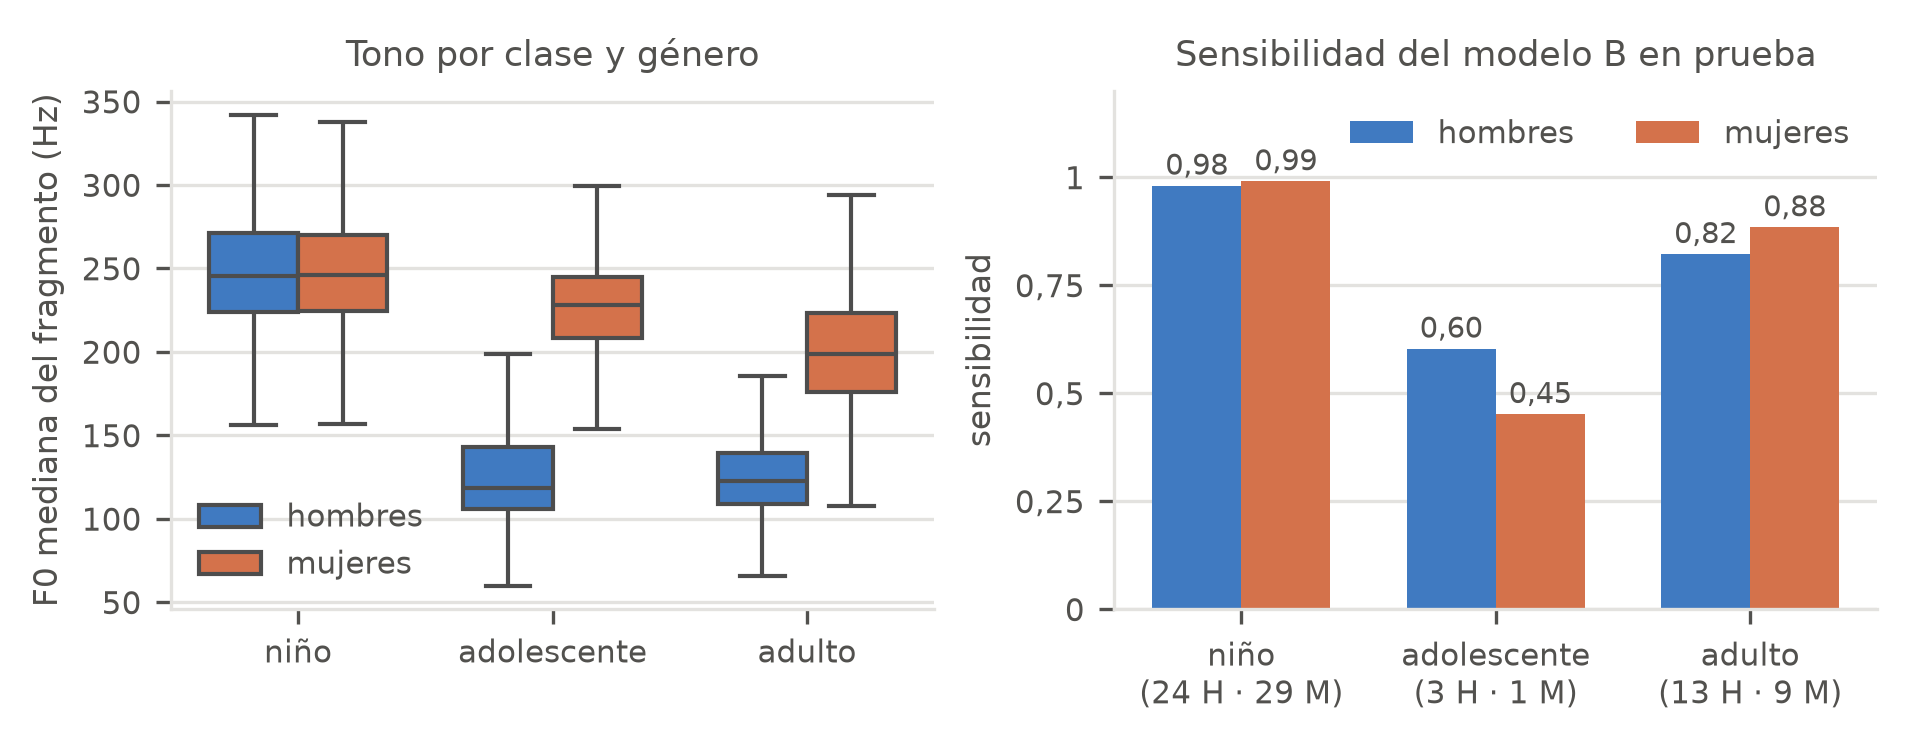
\includegraphics[width=\linewidth]{figuras/genero_tono_sensibilidad.png}
\caption{Izquierda: tono mediano de cada fragmento por clase y género, en todo el conjunto. Derecha: sensibilidad del modelo B por clase y género en prueba; entre paréntesis, el número de hablantes de cada género (H = hombres; M = mujeres).}
\label{fig:genero}
\end{figure}

Si el modelo dependiera del tono, debería equivocarse más con las mujeres. Ocurre lo contrario. La tabla~\ref{tab:genero_modelo} muestra a qué clase asigna el modelo B los fragmentos de prueba de cada grupo: cada fila suma 1 y la diagonal (en negritas) es la sensibilidad. Las mujeres adultas se reconocen como adultas en el 88,4\,\% de los casos, frente al 82,2\,\% de los hombres adultos, y el AUC para separar menores de adultos es de 0,984 en mujeres y de 0,908 en hombres. El error del modelo es masculino: casi tres de cada cuatro fragmentos adolescentes del entrenamiento son de hombres, así que el modelo parece haber aprendido ``adolescente = hombre joven'' y manda a esa clase al 17,8\,\% de los hombres adultos. En niños no hay diferencia por género (0,98 y 0,99). La sensibilidad para mujeres adolescentes (0,45) no es fiable, porque descansa en un único grupo de prueba.

\begin{table}[H]
\centering
\caption{Modelo B en prueba: proporción de cada grupo asignada a cada clase (las filas suman 1) y AUC menor frente a adulto por género.}
\label{tab:genero_modelo}
\small
\begin{tabular}{@{}llccccc@{}}
\toprule
& & \multicolumn{3}{c}{\textbf{Clase predicha}} & & \\
\cmidrule(lr){3-5}
\textbf{Clase real} & \textbf{Género} & \textbf{Niño} & \textbf{Adolescente} & \textbf{Adulto} & \textbf{Fragmentos} & \textbf{Hablantes} \\
\midrule
Niño        & Hombres & \textbf{0,980} & 0,011 & 0,009 & 661 & 24 \\
            & Mujeres & \textbf{0,991} & 0,002 & 0,007 & 846 & 29 \\
Adolescente & Hombres & 0,006 & \textbf{0,603} & 0,391 & 650 & 3 \\
            & Mujeres & 0,016 & \textbf{0,452} & 0,532 & 62 & 1 \\
Adulto      & Hombres & 0,000 & 0,178 & \textbf{0,822} & 871 & 13 \\
            & Mujeres & 0,000 & 0,116 & \textbf{0,884} & 578 & 9 \\
\midrule
\multicolumn{7}{@{}l}{AUC menor frente a adulto: hombres 0,908 (2\,182 fragmentos); mujeres 0,984 (1\,486 fragmentos)} \\
\bottomrule
\end{tabular}
\end{table}

Para medir el efecto de estas diferencias en las alertas, se formaron 3\,000 pares al azar de fragmentos de prueba para cada combinación de clase y género, y se les aplicó la fórmula de riesgo del sistema. La tabla~\ref{tab:genero_riesgo} muestra el riesgo medio y el porcentaje de pares que alcanzan alerta alta y alerta media o alta. Una pareja niño--adulto genera alerta alta algo más a menudo cuando el adulto es mujer (84,5\,\%) que cuando es hombre (79,8\,\%), así que el sistema no deja escapar más casos con mujeres. Entre dos adultos, en cambio, el sesgo masculino del modelo genera más falsas alertas medias: el 28,8\,\% de los pares de hombres alcanza riesgo medio, frente al 20,0\,\% de los pares de mujeres. Ninguna pareja de adultos llega a alerta alta.

\begin{table}[H]
\centering
\caption{Riesgo en 3\,000 pares al azar de fragmentos de prueba por combinación de clase y género (H = hombre; M = mujer).}
\label{tab:genero_riesgo}
\small
\begin{tabular}{@{}lccc@{}}
\toprule
\textbf{Pareja} & \textbf{Riesgo medio} & \textbf{Alerta alta} & \textbf{Alerta media o alta} \\
\midrule
Niño + hombre adulto          & 0,602 & 79,8\,\% & 82,2\,\% \\
Niño + mujer adulta           & 0,624 & 84,5\,\% & 86,8\,\% \\
Adolescente H + hombre adulto & 0,244 & 0,7\,\%  & 56,7\,\% \\
Adolescente M + mujer adulta  & 0,231 & 1,6\,\%  & 47,8\,\% \\
Hombre adulto + hombre adulto & 0,167 & 0,0\,\%  & 28,8\,\% \\
Hombre adulto + mujer adulta  & 0,162 & 0,0\,\%  & 26,2\,\% \\
Mujer adulta + mujer adulta   & 0,147 & 0,0\,\%  & 20,0\,\% \\
\bottomrule
\end{tabular}
\end{table}

Por último, el detector de moduladores mantiene las falsas alarmas bajas en todos los grupos, con un máximo de 1,4\,\% (hombres y mujeres adultos, con y sin canal). Su sensibilidad sí varía con el género y la dirección del cambio cuando hay canal: baja a 0,68 en mujeres a las que se les bajó el tono y a 0,73 en hombres a los que se les subió, frente a 0,83 a 0,87 en los demás casos. Con solo 34 a 183 voces moduladas por grupo, son diferencias que conviene vigilar más que conclusiones firmes.

\subsection{Conversaciones simuladas}

Para probar el sistema completo se armaron conversaciones alternando turnos de hablantes de prueba, con pausas de $0{,}4\,\mathrm{s}$, y se generaron 20 por escenario. La tabla~\ref{tab:simuladas} muestra, para cada escenario, el riesgo medio, el porcentaje de conversaciones con alerta alta y el número medio de hablantes que detectó la diarización frente al número real; la figura~\ref{fig:simuladas} muestra la distribución completa del riesgo.

\begin{table}[H]
\centering
\caption{Resultados del flujo completo con conversaciones simuladas (20 por escenario).}
\label{tab:simuladas}
\small
\begin{tabular}{@{}lccc@{}}
\toprule
\textbf{Escenario} & \textbf{Riesgo medio} & \textbf{Alertas altas} & \textbf{Hablantes detectados (reales)} \\
\midrule
Niño + adulto        & 0,587 & 80\,\% & 3,3 (2) \\
Adolescente + adulto & 0,223 & 0\,\%  & 2,1 (2) \\
Adulto + adulto      & 0,188 & 0\,\%  & 2,4 (2) \\
Niño + niño          & 0,111 & 0\,\%  & 3,9 (2) \\
Adulto solo          & 0,068 & 0\,\%  & 1,2 (1) \\
\bottomrule
\end{tabular}
\end{table}

\begin{figure}[H]
\centering
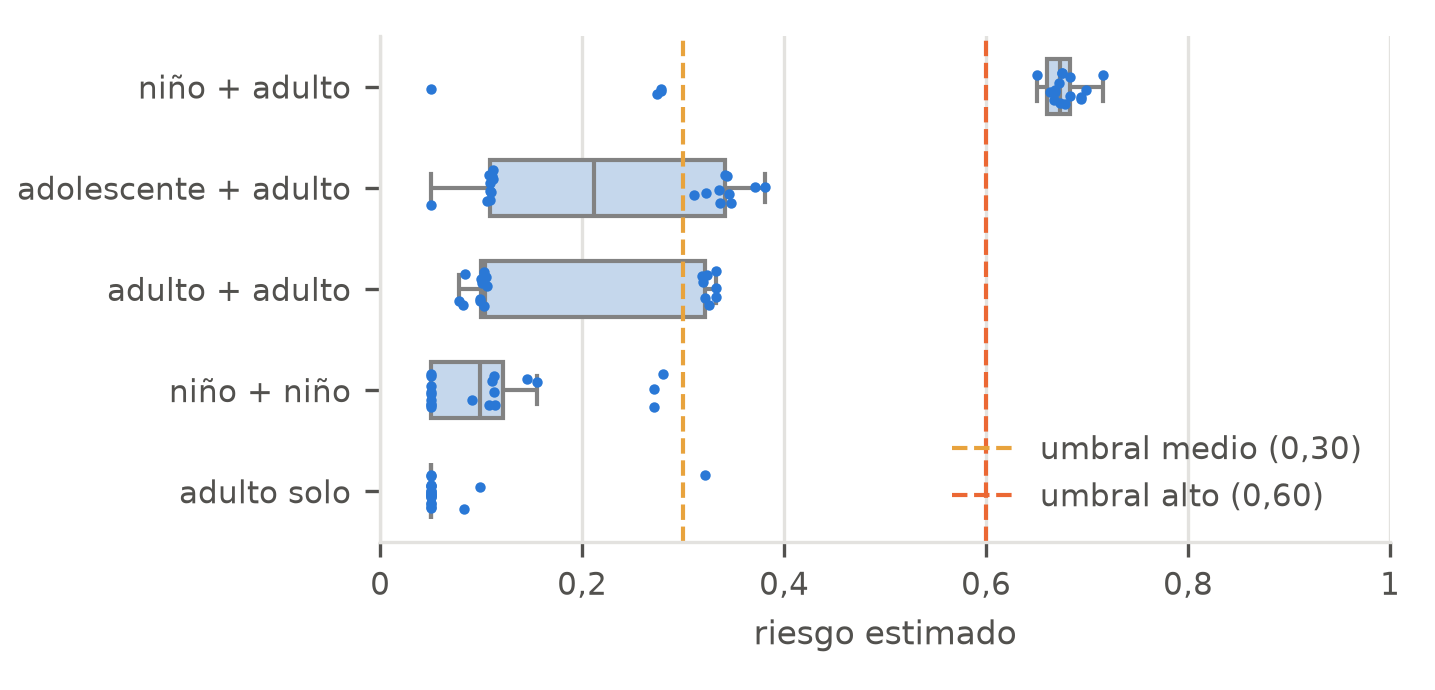
\includegraphics[width=0.75\linewidth]{figuras/riesgo_escenarios_simulados.png}
\caption{Distribución del riesgo estimado en las conversaciones simuladas, por escenario. Cada punto es una conversación; las líneas punteadas marcan los umbrales de riesgo medio (0,30) y alto (0,60).}
\label{fig:simuladas}
\end{figure}

Las conversaciones entre niño y adulto generan alerta alta en el 80\,\% de los casos, y ningún otro escenario llega a alerta alta, aunque algunas conversaciones adolescente + adulto y adulto + adulto alcanzan riesgo medio. La diarización cuenta hablantes de más cuando hay niños, porque cada fragmento sintetizado suena como una voz distinta; eso reparte al niño entre varios hablantes falsos y baja el riesgo medio. Indicar el número de participantes corrige el problema: con dos hablantes indicados, una conversación de prueba niño--adulto obtuvo 71\,\% (alto), con el niño identificado al 86\,\% y el adulto al 84\,\%. Por último, el escenario adolescente + adulto casi nunca alerta, consecuencia directa de la baja sensibilidad para adolescentes.

\subsection{Detector de moduladores de voz}

Antes de evaluar el detector se comprobó que el problema existe: en la API, un adulto de prueba con el tono subido 1,45 veces por el cambio de tono simple fue clasificado como \emph{niño}. La tabla~\ref{tab:detector_limpio} muestra el detector limpio sobre la prueba sin degradar, con 4\,100 fragmentos de los que 376 están modulados. La parte superior compara las dos cabezas; la SVM, elegida en validación con $C = 3$ y umbral 0,43, es mejor en todas las métricas. La parte inferior desglosa la SVM: a la izquierda, la sensibilidad para cada modulador, y a la derecha, la tasa de falsas alarmas en voces originales de cada clase.

\begin{table}[H]
\centering
\caption{Detector limpio en el conjunto de prueba sin degradar (4\,100 fragmentos, 376 modulados).}
\label{tab:detector_limpio}
\small
\begin{tabular}{@{}lccccc@{}}
\toprule
\textbf{Cabeza} & \textbf{Precisión} & \textbf{Sensibilidad} & \textbf{F1} & \textbf{AUC} & \textbf{Prec. media} \\
\midrule
SVM (elegida en validación) & \textbf{0,976} & \textbf{0,851} & \textbf{0,909} & \textbf{0,992} & \textbf{0,962} \\
Regresión logística         & 0,860 & 0,782 & 0,819 & 0,979 & 0,894 \\
\bottomrule
\end{tabular}

\vspace{6pt}
\begin{tabular}{@{}lcc@{\hspace{2.2em}}lcc@{}}
\toprule
\multicolumn{3}{@{}l}{\textbf{Sensibilidad por modulador}} & \multicolumn{3}{l@{}}{\textbf{Falsas alarmas en voces originales}} \\
\midrule
Cambio de tono simple & 0,950 & ($n=139$) & Niños        & 0,1\,\% & ($n=1\,507$) \\
Praat                 & 0,866 & ($n=112$) & Adolescentes & 0,1\,\% & ($n=712$) \\
WORLD (no visto)      & 0,728 & ($n=125$) & Adultos      & 0,4\,\% & ($n=1\,505$) \\
\bottomrule
\end{tabular}
\end{table}

Con audio limpio casi no hay falsas alarmas: solo 1 de cada 1\,000 niños originales se marca como modulado, aunque se temía que el habla sintetizada de ENNI pareciera ``modificada''. El detector generaliza al modulador que nunca vio, pero con pérdida: WORLD se detecta en el 72,8\,\% de los casos, frente al 95,0\,\% del cambio de tono simple. La dirección del cambio no importa: se detecta el 84,7\,\% de las voces subidas y el 86,3\,\% de las bajadas.

La tabla~\ref{tab:acople} compara el detector limpio con el acoplado, cada uno sobre la prueba limpia y sobre la misma prueba con canal. Las dos primeras filas muestran que, sin acople, el canal rompe el detector: con audio sucio pierde 0,17 de F1 (de 0,909 a 0,743) y deja escapar a un tercio de las voces moduladas. Las dos últimas muestran que el detector acoplado (SVM con $C = 1$ y umbral 0,37) recupera la mitad de esa pérdida con canal (F1 de 0,829) y queda prácticamente igual con audio limpio (0,902 frente a 0,909). Por eso el sistema despliega el detector acoplado.

\begin{table}[H]
\centering
\caption{Detector limpio frente a acoplado, en prueba sin degradar y con canal (cada versión: 4\,100 fragmentos, 376 modulados).}
\label{tab:acople}
\small
\begin{tabular}{@{}llccccc@{}}
\toprule
\textbf{Detector} & \textbf{Audio de prueba} & \textbf{Precisión} & \textbf{Sensibilidad} & \textbf{F1} & \textbf{AUC} & \textbf{Prec. media} \\
\midrule
Limpio   & limpio    & 0,976 & 0,851 & 0,909 & 0,992 & 0,962 \\
Limpio   & con canal & 0,834 & 0,670 & 0,743 & 0,965 & 0,848 \\
\midrule
Acoplado & limpio    & 0,950 & 0,859 & 0,902 & 0,992 & 0,955 \\
Acoplado & con canal & 0,900 & 0,769 & 0,829 & 0,978 & 0,904 \\
\bottomrule
\end{tabular}
\end{table}

La figura~\ref{fig:moduladores} muestra el puntaje del detector acoplado por grupo en la prueba con canal, y la tabla~\ref{tab:acople_desglose} lo desglosa igual que la tabla~\ref{tab:detector_limpio}. El detector \textbf{no aprendió el atajo} ``audio sucio = modulado'': en las voces originales, la tasa de falsas alarmas apenas pasa de 0,5\,\% sin canal a 0,9\,\% con canal, y en niños se queda en 0,6\,\%. Con canal sigue habiendo un hueco: casi una de cada cuatro voces moduladas pasa sin marcar, y casi un tercio en el modulador no visto. Los cambios suaves escapan más: en la API, una copia de Praat con factor 1,23 obtuvo una probabilidad de 0,13, por debajo del umbral.

\begin{table}[H]
\centering
\caption{Detector acoplado en la prueba con canal: sensibilidad por modulador y falsas alarmas por clase.}
\label{tab:acople_desglose}
\small
\begin{tabular}{@{}lcc@{\hspace{2.2em}}lcc@{}}
\toprule
\multicolumn{3}{@{}l}{\textbf{Sensibilidad por modulador}} & \multicolumn{3}{l@{}}{\textbf{Falsas alarmas en voces originales}} \\
\midrule
Cambio de tono simple & 0,849 & ($n=139$) & Niños        & 0,6\,\% & ($n=1\,507$) \\
Praat                 & 0,759 & ($n=112$) & Adolescentes & 0,7\,\% & ($n=712$) \\
WORLD (no visto)      & 0,688 & ($n=125$) & Adultos      & 1,2\,\% & ($n=1\,505$) \\
\bottomrule
\end{tabular}
\end{table}

\begin{figure}[H]
\centering
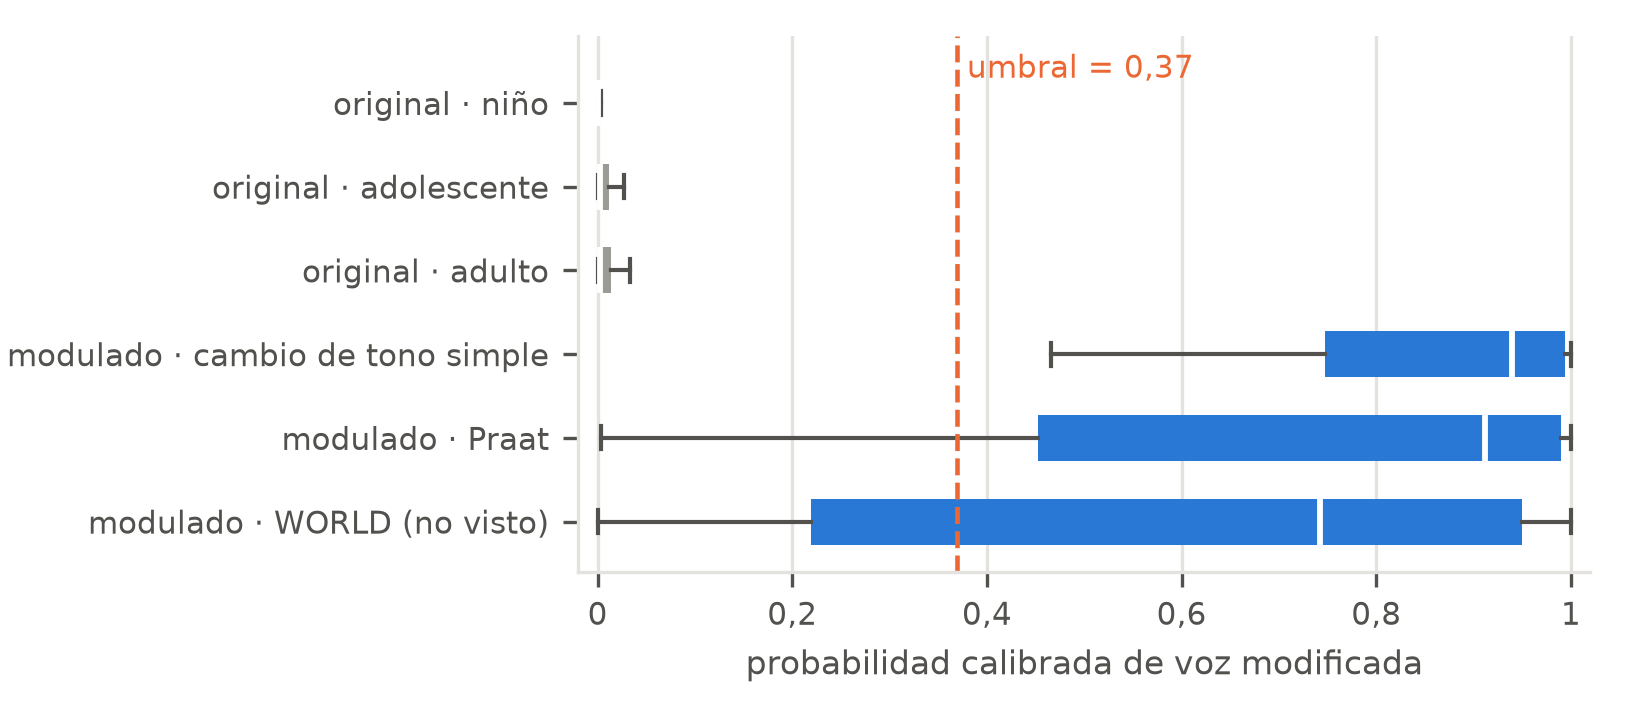
\includegraphics[width=0.85\linewidth]{figuras/detector_moduladores.png}
\caption{Detector acoplado (el desplegado): probabilidad de voz modificada por grupo en la prueba con canal. Las voces originales quedan pegadas a 0; las cajas muestran el rango intercuartil.}
\label{fig:moduladores}
\end{figure}

\subsection{Pruebas del sistema}

Además de la evaluación de los modelos, se verificó el sistema como software. La tabla~\ref{tab:pruebas} resume cada prueba, qué verifica y su resultado; todas se superaron.

\begin{table}[H]
\centering
\caption{Resumen de pruebas.}
\label{tab:pruebas}
\small
\begin{tabularx}{\linewidth}{@{}>{\raggedright\arraybackslash}p{3.8cm}L>{\raggedright\arraybackslash}p{3.2cm}@{}}
\toprule
\textbf{Prueba} & \textbf{Qué verifica} & \textbf{Resultado} \\
\midrule
Pruebas unitarias (15 casos) & Fronteras de edad; riesgo de 90\,\% para niño + adulto y de 60\,\% para adolescente + adulto; piso sin pareja menor--adulto; escalado con la incertidumbre & 15/15 correctas \\
Ausencia de fuga de hablantes & Ningún hablante en dos particiones, tampoco en las copias moduladas & Verificada \\
Calidad de datos & Eliminación de fragmentos mudos y verificación de etiquetas & 13 mudos eliminados \\
Entrenamiento completo & Todo el cuaderno de principio a fin con los datos completos & Sin errores \\
Robustez al canal & Rendimiento con audio degradado por los doce filtros & F1 de 0,812 a 0,793 \\
Detector de moduladores & Sensibilidad por tipo, falsas alarmas por clase, con y sin canal; atajo ``audio sucio = modulado'' & F1 de 0,829 con canal \\
API local y en contenedor & Respuestas idénticas en ambos entornos, aviso presente, bandera activa en voces moduladas de prueba & Correcta \\
\bottomrule
\end{tabularx}
\end{table}

%=====================================================================
\section{Conclusiones}
%=====================================================================

Este trabajo mostró que es posible estimar, solo con la voz y sin analizar el contenido, si en una conversación hablan una persona menor de edad y una adulta. El mejor modelo, vectores de hablante ECAPA-TDNN con una máquina de vectores de soporte, alcanza un F1-macro de 0,812 por fragmento y separa menores de adultos con un AUC de 0,944. En el flujo completo, las conversaciones simuladas entre un niño y un adulto generan alerta alta en el 80\,\% de los casos, mientras que ningún escenario sin pareja menor--adulto llega a ese nivel.

La comparación controlada de seis modelos deja tres lecciones. La primera es que la representación importa más que el clasificador: los vectores de hablante preentrenados superan a los rasgos acústicos clásicos, MFCC incluidos, y a una red autosupervisada más grande como WavLM, con un costo de solo $31\,\mathrm{ms}$ por fragmento. La segunda es que la frontera entre adolescentes y adultos no es lineal, lo que favorece a los clasificadores no paramétricos: con la misma representación, la SVM supera al bosque aleatorio, y la regresión logística sobre rasgos acústicos casi no reconoce adolescentes. La tercera es que distinguir niños de adultos es relativamente fácil, pero distinguir adolescentes de adultos sigue siendo el reto abierto, porque sus voces se superponen desde el punto de vista fisiológico; en el sistema esto se traduce en que casi nunca alerta por una pareja adolescente--adulto.

El trabajo con filtros y moduladores mostró que el sistema puede prepararse para las condiciones reales de un chat de voz. Entrenado con doce filtros que imitan el canal y el fondo de un videojuego, el modelo de edad pierde solo 0,019 de F1-macro con audio degradado, y el análisis de los filtros reveló que el riesgo no está en el tono sino en los formantes, que el canal telefónico borra y el ruido inventa. Un modulador de voz, en cambio, sí puede hacer pasar a un adulto por niño. El detector de voz modificada, una cabeza ligera sobre el mismo vector ECAPA, lo mitiga sin costo de extracción, y su versión acoplada ---primero el modulador, después el canal, con el mismo trato para originales y modulados--- recupera la mitad de lo que el canal le quitaba a un detector entrenado con audio limpio, sin aprender el atajo ``audio sucio = modulado''.

El análisis por género corrigió una intuición. Por fisiología, el tono confunde a las mujeres adultas con niños, pero el modelo no depende solo del tono: separa mejor a menores y adultos en mujeres que en hombres, y su error dominante es tomar a hombres adultos por adolescentes, un reflejo de que casi tres de cada cuatro fragmentos adolescentes de entrenamiento son de hombres. En el riesgo, esto no reduce las alertas niño--adulto con mujeres, pero sí produce más alertas medias en conversaciones entre hombres adultos. La lección es que el desbalance del corpus pesa más que la fisiología, y que cualquier corpus futuro debe equilibrar el género dentro de cada clase.

Los resultados tienen límites claros. Todos los niños provienen de habla sintetizada, cada clase sale de un solo corpus y hay muy pocos grupos de adolescentes, así que el desempeño con niños puede estar inflado y la sensibilidad para adolescentes es imprecisa. La evaluación del flujo completo y del detector se hizo con conversaciones y moduladores simulados. Por eso el sistema debe entenderse como lo que es: una alerta para priorizar revisión humana, que protege la privacidad por construcción ---no transcribe, no guarda audio y solo produce probabilidades de edad--- y que antes de cualquier uso real necesita datos de niños reales grabados en las mismas condiciones que los adultos y validación con conversaciones reales.

%=====================================================================
\section{Trabajo a futuro}
%=====================================================================

Los resultados muestran que la propuesta es viable, pero el sistema todavía no está listo para un uso real. La tabla~\ref{tab:futuro} resume sus limitaciones conocidas: cada fila indica una limitación, su efecto en los resultados y la mejora que proponemos.

\begin{table}[H]
\centering
\caption{Limitaciones conocidas y mejoras propuestas.}
\label{tab:futuro}
\small
\begin{tabularx}{\linewidth}{@{}>{\raggedright\arraybackslash}p{4cm}L>{\raggedright\arraybackslash}p{4.3cm}@{}}
\toprule
\textbf{Limitación} & \textbf{Efecto} & \textbf{Mejora} \\
\midrule
Todos los niños provienen de habla sintetizada & El rendimiento con niños puede estar inflado & Corpus con niños y adultos reales en el mismo canal (speechocean762, MyST, CSLU Kids) \\
Pocos adolescentes (25 grupos) & Sensibilidad de 0,59; casi no hay alertas adolescente--adulto & Más datos de adolescentes con edad exacta \\
\emph{Teens} en Common Voice incluye 18 y 19 años & Etiquetas ruidosas & Corpus con edad exacta \\
Solo inglés & Rendimiento desconocido en español & Añadir voces en español \\
Diarización ligera & Cuenta hablantes de más con voces infantiles & Diarización neuronal (pyannote, NeMo) \\
Evaluación con conversaciones simuladas & Resultados optimistas & Validación con conversaciones reales anotadas, con consentimiento \\
Canal y fondos simulados & Con canal, casi una de cada cuatro voces moduladas pasa sin marcar & Grabaciones reales de chats de voz y fondos reales de partidas \\
Solo tres moduladores simulados & Un modulador comercial o neuronal puede escapar (WORLD, no visto: 0,69 con canal) & Moduladores comerciales y conversión de voz neuronal \\
Adolescentes mayoritariamente hombres (un solo grupo de mujeres en prueba) & El modelo confunde hombres adultos con adolescentes; la sensibilidad en mujeres adolescentes no es medible & Equilibrar el género dentro de cada clase y reportar las métricas por género \\
Formantes poco fiables & El estimador por predicción lineal casi no distingue hombres de mujeres & Estimar formantes con Praat o filtrar cuadros sin voz clara \\
\bottomrule
\end{tabularx}
\end{table}

Además de esas mejoras, hay tres líneas de trabajo. La primera es el ajuste fino de WavLM: con más datos de menores, el siguiente paso natural es ajustarlo en lugar de usarlo congelado. La segunda es la calibración de umbrales: los pesos y umbrales del riesgo se fijaron por diseño y deben recalibrarse con conversaciones reales, documentando cada cambio. La tercera son las condiciones para un despliegue real, que requeriría base legal, aviso o consentimiento adecuado, una evaluación de impacto en protección de datos y un equipo de revisión humana especializada. Ninguna acción con consecuencias debe acoplarse automáticamente al puntaje, y debe asumirse que la mayoría de las alertas corresponderán a conversaciones legítimas.

%=====================================================================
\section{Declaración de uso de IA}
%=====================================================================

En la elaboración de este trabajo se usaron dos herramientas de inteligencia artificial generativa como apoyo. Gemini (Google) se usó como apoyo en la investigación, principalmente para la búsqueda inicial de trabajos relacionados, de estadísticas sobre \gr{} en línea y de corpus de voz infantil disponibles; este apoyo se refleja en la Introducción, los Trabajos relacionados y el Marco teórico. Claude (Anthropic) se usó como apoyo con el formato \LaTeX{} del reporte ---la estructura del documento, las tablas, las figuras y la bibliografía--- y para consultas puntuales de código durante la implementación.

Las fuentes sugeridas durante la investigación se consultaron y verificaron directamente antes de citarse. El diseño del sistema, la selección de los datos, el entrenamiento y la evaluación de los modelos, el análisis de los resultados y las conclusiones son trabajo del equipo.

%=====================================================================
\begin{thebibliography}{99}
\small

\bibitem{commonvoice2020} R.~Ardila et~al. \emph{Common Voice: A Massively-Multilingual Speech Corpus}. \emph{Proceedings of LREC}, 2020.

\bibitem{bahari2014} M.~H.~Bahari, M.~McLaren, H.~Van~hamme y D.~A.~van~Leeuwen. \emph{Speaker age estimation using i-vectors}. \emph{Engineering Applications of Artificial Intelligence}, 34:99--108, 2014.

\bibitem{praat} P.~Boersma y D.~Weenink. \emph{Praat: doing phonetics by computer}. \url{https://www.praat.org}; usado mediante Y.~Jadoul, B.~Thompson y B.~de~Boer, \emph{Introducing Parselmouth: A Python interface to Praat}, \emph{Journal of Phonetics}, 71:1--15, 2018.

\bibitem{pyannote2020} H.~Bredin et~al. \emph{pyannote.audio: neural building blocks for speaker diarization}. \emph{IEEE ICASSP}, 2020.

\bibitem{rf2001} L.~Breiman. \emph{Random Forests}. \emph{Machine Learning}, 45:5--32, 2001.

\bibitem{burkhardt2023} F.~Burkhardt, J.~Wagner, H.~Wierstorf, F.~Eyben y B.~Schuller. \emph{Speech-based age and gender prediction with transformers}. \emph{ITG Conference on Speech Communication}, 2023.

\bibitem{wavlm2022} S.~Chen et~al. \emph{WavLM: Large-Scale Self-Supervised Pre-Training for Full Stack Speech Processing}. \emph{IEEE Journal of Selected Topics in Signal Processing}, 16(6), 2022.

\bibitem{svm1995} C.~Cortes y V.~Vapnik. \emph{Support-vector networks}. \emph{Machine Learning}, 20:273--297, 1995.

\bibitem{davis1980} S.~Davis y P.~Mermelstein. \emph{Comparison of parametric representations for monosyllabic word recognition in continuously spoken sentences}. \emph{IEEE Transactions on Acoustics, Speech, and Signal Processing}, 28(4):357--366, 1980.

\bibitem{ecapa2020} B.~Desplanques, J.~Thienpondt y K.~Demuynck. \emph{ECAPA-TDNN: Emphasized Channel Attention, Propagation and Aggregation in TDNN Based Speaker Verification}. \emph{Interspeech}, 2020.

\bibitem{ebrahimi2016} M.~Ebrahimi, C.~Y.~Suen y O.~Ormandjieva. \emph{Detecting predatory conversations in social media by deep convolutional neural networks}. \emph{Digital Investigation}, 18:33--49, 2016.

\bibitem{edpb2022} EDPB y EDPS. \emph{Joint Opinion 4/2022 on the Proposal for a Regulation laying down rules to prevent and combat child sexual abuse}, 28 de julio de 2022. \url{https://edps.europa.eu/data-protection/our-work/publications/edps-edpb-joint-opinions/2022-07-28-joint-opinion-42022-regulation-european-parliament-and-council-rules-prevent-and-combat-child-sexual-abuse_en}

\bibitem{fant1960} G.~Fant. \emph{Acoustic Theory of Speech Production}. Mouton, La Haya, 1960.

\bibitem{fawcett2006} T.~Fawcett. \emph{An introduction to ROC analysis}. \emph{Pattern Recognition Letters}, 27(8):861--874, 2006.

\bibitem{friedman2001} J.~H.~Friedman. \emph{Greedy function approximation: A gradient boosting machine}. \emph{Annals of Statistics}, 29(5):1189--1232, 2001.

\bibitem{furui1986} S.~Furui. \emph{Speaker-independent isolated word recognition using dynamic features of speech spectrum}. \emph{IEEE Transactions on Acoustics, Speech, and Signal Processing}, 34(1):52--59, 1986.

\bibitem{garnerin2019} M.~Garnerin, S.~Rossato y L.~Besacier. \emph{Gender representation in French broadcast corpora and its impact on ASR performance}. \emph{Proceedings of the 1st International Workshop on AI for Smart TV Content Production, Access and Delivery (AI4TV)}, ACM, 2019.

\bibitem{ghahremani2018} P.~Ghahremani, P.~S.~Nidadavolu, N.~Chen, J.~Villalba, D.~Povey, S.~Khudanpur y N.~Dehak. \emph{End-to-end deep neural network age estimation}. \emph{Interspeech}, 2018.

\bibitem{hillenbrand1995} J.~Hillenbrand, L.~A.~Getty, M.~J.~Clark y K.~Wheeler. \emph{Acoustic characteristics of American English vowels}. \emph{Journal of the Acoustical Society of America}, 97(5):3099--3111, 1995.

\bibitem{pan2012} G.~Inches y F.~Crestani. \emph{Overview of the International Sexual Predator Identification Competition at PAN-2012}. \emph{CLEF 2012 Evaluation Labs and Workshop}, 2012.

\bibitem{inegi2025} INEGI. Módulo sobre Ciberacoso (MOCIBA) 2024, comunicado de prensa 76/25, 17 de julio de 2025. \url{https://www.inegi.org.mx/programas/mociba/2024/}

\bibitem{enniHF} jsun39. \emph{enni-child-speech-synthesis} (conjunto de datos). Hugging Face. \url{https://huggingface.co/datasets/jsun39/enni-child-speech-synthesis}

\bibitem{ko2015} T.~Ko, V.~Peddinti, D.~Povey y S.~Khudanpur. \emph{Audio augmentation for speech recognition}. \emph{Interspeech}, 2015.

\bibitem{lee1999} S.~Lee, A.~Potamianos y S.~Narayanan. \emph{Acoustics of children's speech: Developmental changes of temporal and spectral parameters}. \emph{Journal of the Acoustical Society of America}, 105(3):1455--1468, 1999.

\bibitem{metze2007} F.~Metze, J.~Ajmera, R.~Englert, U.~Bub, F.~Burkhardt, J.~Stegmann, C.~Müller, R.~Huber, B.~Andrassy, J.~G.~Bauer y B.~Littel. \emph{Comparison of four approaches to age and gender recognition for telephone applications}. \emph{IEEE ICASSP}, 2007.

\bibitem{world2016} M.~Morise, F.~Yokomori y K.~Ozawa. \emph{WORLD: A Vocoder-Based High-Quality Speech Synthesis System for Real-Time Applications}. \emph{IEICE Transactions on Information and Systems}, E99-D(7):1877--1884, 2016.

\bibitem{ncmec2025} National Center for Missing \& Exploited Children. \emph{NCMEC Releases New Data: 2024 in Numbers}, 2025. \url{https://www.missingkids.org/blog/2025/ncmec-releases-new-data-2024-in-numbers}

\bibitem{nspcc2025} NSPCC. \emph{Data shows how criminals are using private messaging platforms to manipulate and groom children}, noviembre de 2025. \url{https://www.nspcc.org.uk/about-us/news-opinion/2025/data-shows-how-criminals-are-using-private-messaging-platforms-to-manipulate-and-groom-children/}

\bibitem{park2022} T.~J.~Park, N.~Kanda, D.~Dimitriadis, K.~J.~Han, S.~Watanabe y S.~Narayanan. \emph{A review of speaker diarization: Recent advances with deep learning}. \emph{Computer Speech \& Language}, 72:101317, 2022.

\bibitem{sklearn2011} F.~Pedregosa et~al. \emph{Scikit-learn: Machine Learning in Python}. \emph{Journal of Machine Learning Research}, 12:2825--2830, 2011.

\bibitem{platt1999} J.~Platt. \emph{Probabilistic outputs for support vector machines and comparisons to regularized likelihood methods}. \emph{Advances in Large Margin Classifiers}, 1999.

\bibitem{speechbrain2021} M.~Ravanelli et~al. \emph{SpeechBrain: A General-Purpose Speech Toolkit}. arXiv:2106.04624, 2021.

\bibitem{enni2005} P.~Schneider, R.~V.~Dubé y D.~Hayward. \emph{The Edmonton Narrative Norms Instrument}. \emph{University of Alberta}, 2005.

\bibitem{schuller2010} B.~Schuller, S.~Steidl, A.~Batliner, F.~Burkhardt, L.~Devillers, C.~Müller y S.~Narayanan. \emph{The INTERSPEECH 2010 Paralinguistic Challenge}. \emph{Interspeech}, 2010.

\bibitem{xvector2018} D.~Snyder, D.~Garcia-Romero, G.~Sell, D.~Povey y S.~Khudanpur. \emph{X-vectors: Robust DNN embeddings for speaker recognition}. \emph{IEEE ICASSP}, 2018.

\bibitem{tatman2017} R.~Tatman. \emph{Gender and dialect bias in YouTube's automatic captions}. \emph{Proceedings of the First ACL Workshop on Ethics in Natural Language Processing}, 53--59, 2017.

\bibitem{thorn2025} Thorn. \emph{What the 2024 NCMEC CyberTipline Report Says About Child Safety}, 2025. \url{https://www.thorn.org/blog/what-the-2024-ncmec-cybertipline-report-says-about-child-safety/}

\bibitem{titze1989} I.~R.~Titze. \emph{Physiologic and acoustic differences between male and female voices}. \emph{Journal of the Acoustical Society of America}, 85(4):1699--1707, 1989.

\bibitem{todisco2019} M.~Todisco, X.~Wang, V.~Vestman, M.~Sahidullah, H.~Delgado, A.~Nautsch, J.~Yamagishi, N.~Evans, T.~Kinnunen y K.~A.~Lee. \emph{ASVspoof 2019: Future horizons in spoofed and fake audio detection}. \emph{Interspeech}, 2019.

\bibitem{villatoro2012} E.~Villatoro-Tello, A.~Juárez-González, H.~J.~Escalante, M.~Montes-y-Gómez y L.~Villaseñor-Pineda. \emph{A two-step approach for effective detection of misbehaving users in chats}. \emph{CLEF 2012 Evaluation Labs and Workshop}, 2012.

\bibitem{weprotect2023} WeProtect Global Alliance. \emph{Global Threat Assessment 2023}. \url{https://www.weprotect.org/global-threat-assessment-23/}

\bibitem{whittle2013} H.~Whittle, C.~Hamilton-Giachritsis, A.~Beech y G.~Collings. \emph{A review of online grooming: Characteristics and concerns}. \emph{Aggression and Violent Behavior}, 18(1):62--70, 2013.

\bibitem{wu2014} H.~Wu, Y.~Wang y J.~Huang. \emph{Identification of electronic disguised voices}. \emph{IEEE Transactions on Information Forensics and Security}, 9(3):489--500, 2014.

\bibitem{superb2021} S.~Yang et~al. \emph{SUPERB: Speech processing Universal PERformance Benchmark}. \emph{Interspeech}, 2021.

\end{thebibliography}

\end{document}
